\title{Quarks to Cosmos: Particles and Plasma in\\ 
 Cosmological evolution}

\author{
Johann Rafelski${}^1$\orc{\orcA}\thanks{Corresponding author 
\email{johannr@arizona.edu}}, 
Jeremiah Birrell${}^{1,2}$\orc{\orcE}, 
Christopher Grayson${}^1$\orc{\orcF}, 
\newline Andrew Steinmetz${}^1$\orc{\orcC}, 
Cheng Tao Yang${}^1$\orc{\orcB}
}

\institute{${}^1$Department of Physics, The University of Arizona, Tucson, AZ, 85721, USA\\
${}^2$Department of Mathematics, Texas State University, San Marcos, TX, 78666, USA}

\abstract{We describe in the context of the particle physics (PP) standard model (SM) `PP-SM' the understanding of the primordial properties and composition of the Universe in the temperature range $130\GeV>T>20\keV$. The Universe evolution is described using FLRW cosmology. We present a global view on particle content across time and describe the different evolution eras using deceleration parameter $q$. In the considered temperature range the unknown cold dark matter and dark energy content of $\Lambda\mathrm{CDM}$ have a negligible influence allowing a reliable understanding of physical properties of the Universe based on PP-SM energy-momentum alone. We follow the arrow of time in the expanding and cooling Universe: After the PP-SM heavies $(t, h, W, Z)$ diminish in abundance below $T\simeq 50\GeV$, the PP-SM plasma in the Universe is governed by the strongly interacting Quark-Gluon content. Once the temperature drops below $T\simeq 150\MeV$, quarks and gluons hadronize into strongly interacting matter particles comprising a dense baryon-antibaryon content. Rapid disappearance of baryonic antimatter ensues, which adopting the present day photon-to-baryon ratio completes at $T_\mathrm{B}=38.2\MeV$. We study the ensuing disappearance of strangeness and mesons in general. We show that the different eras defined by particle populations are barely separated from each other with abundance of muons fading out just prior to $T=\mathcal{O}(2.5)\MeV$, the era of emergence of the free-streaming neutrinos. We develop methods allowing the study of the ensuing speed of the Universe expansion as a function of fundamental coupling parameters in the primordial epoch. We discuss the two relevant fundamental constants controlling the decoupling of neutrinos. We subsequently follow the primordial Universe as it passes through the hot dense electron-positron plasma epoch. The high density of positron antimatter disappears near $T=20.3\keV$, well after the Big-Bang Nucleosynthesis era: Nuclear reactions occur in the presence of a highly mobile and relatively strongly interacting electron-positron plasma phase. We apply plasma theory methods to describe the strong screening effects between heavy dust particle (nucleons). We analyze the paramagnetic characteristics of the electron-positron plasma when exposed to an external primordial magnetic field.}
\maketitle
%%%%%%%%%%%%%%%%%%%%%%%%%%%%%%%%%%%%%%%
%\newpage
\setcounter{tocdepth}{3}
\tableofcontents
%%%%%%%%%%%%%%%%%%%%%%%%%%%%%%%%%%%%%%%

%%%%%%%%%%%%%%%%%%%%%%%%%%%%%%%%%%%%%%% 
\section{Introduction}
%%%%%%%%%%%%%%%%%%%%%%%%%%%%%
\subsection{Theoretical models of the primordial Universe}\label{ssec:UniLab}
In this report we explore the connection between particle, nuclear, and plasma physics in the evolution of the Universe. Our work concerns the domain described by the known laws of physics as determined by laboratory experiments.

Our journey in time through the expanding primordial Universe has the objective of understanding how different evolution eras impact each other. We are seeking to gain deeper insights into the fundamental processes that shaped our cosmos, by providing a clearer picture of the Universe's origin and its ongoing expansion. The question we address is how a very hot soup of elementary matter evolves and connects to the normal matter present today, indirectly observed by the elemental ashes of the Big-Bang nucleosynthesis (BBN)\index{Big-Bang!BBN}. 

{\color{black}In this report we report on our  ongoing work on particle and plasma cosmology. Our aim is to create a continuous description of the primordial Universe spanning and connecting different particle and plasma epochs. This allows the reader to understand the physics spanning the entire temperature domain we explore, $130\GeV>T>20\,\mathrm{keV}$. We will define many topics deserving further study: There are many open questions to which this work provides an introduction.}

{\color{black}This manuscript is not a traditional review, as its focus is on our own ongoing work: We aim here to offer a readable report describing and explaining what can appear at times to be a fragmented body of work. A  guide- and time-line how our theoretical insights were gained over the past dozen years is presented in \rapp{list:Works}.}

{\color{black}As appropriate we highlight in \rapp{list:Works} the key results and provide fields of application not yet fully explored. This helps to create a backdrop of knowledge and introduces further areas of study potentially helping to understand the primordial Universe and sharpen prediction of observable quantities today.} 

%%%%%%%%%%%%%%%%%%%%%%%
\para{Dominance of visible radiation and matter in the primordial Universe}
In this report, we aim to connect various eras of cosmological evolution which can be addressed with some confidence in view of the already known particle and nuclear properties as measured experimentally. By analyzing the primordial Universe as a function of time in~\rf{fig:energy:frac} we are exploring the role of particle physics standard model (PP-SM) in the Universe evolution. We snapshot in this report specific epochs in the primordial Universe, and/or on specific physical conditions such as primordial magnetic fields.

%%%%%%%%%%%%%%%%%%%%%%%%%%%%%%%%%%%%
%\begin{sidewaysfigure}
\begin{figure}
%\vspace*{0.62\linewidth}
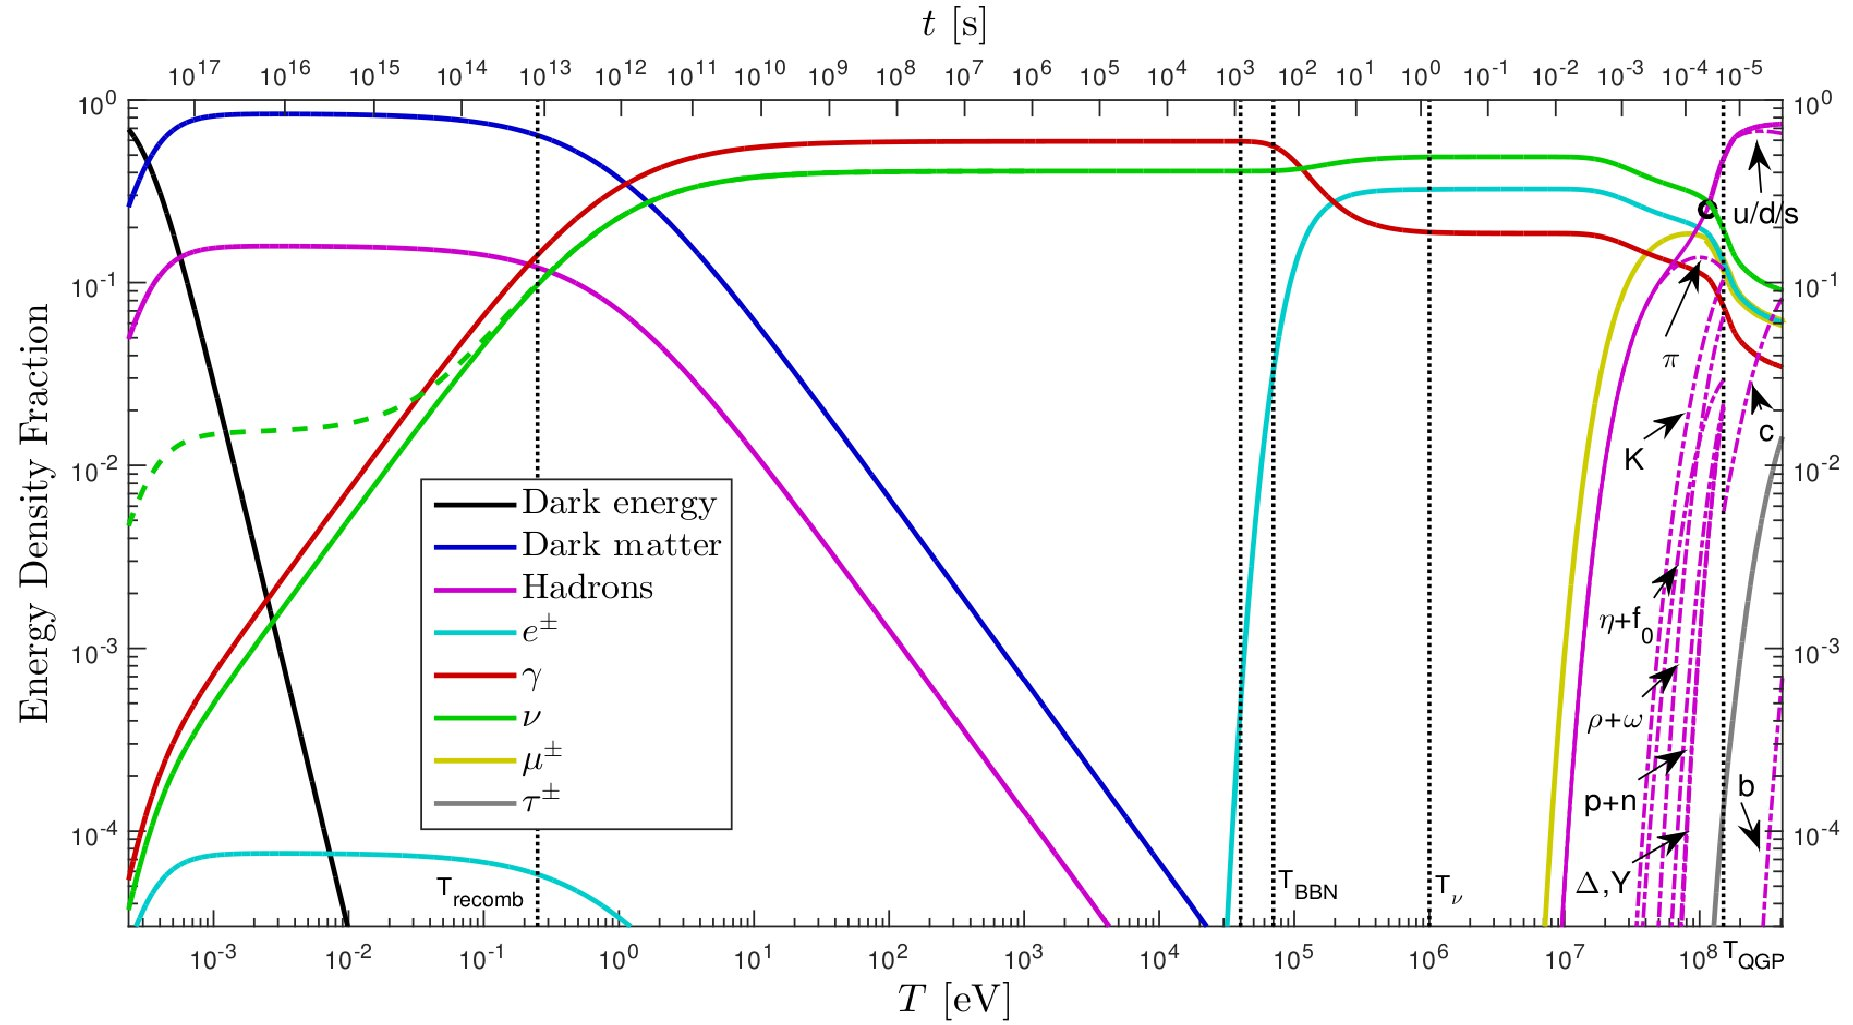
\includegraphics[width=\linewidth]{plots/energyFractions.jpg}\label{fig:energy:frac}
\caption{Evolving in time fractional energy composition of the Universe. See text for discussion. \cccite{Rafelski:2023emw}. \radapt{Birrell:2014ona}.}
% \end{sidewaysfigure}
\end{figure}
%%%%%%%%%%%%%%%%%%%%%%%%%%%%%%%%%%

In the cosmic epoch considered here with temperature above $kT=20\keV$, the present day dominant dark matter and dark energy played a negligible role in the cosmos. The changing energy component composition of the Universe\index{Universe!composition} is illustrated in~\rf{fig:energy:frac}. To create the figure we integrate the Universe backwards in time. The initial condition is the assumed composition of the Universe in the current era: $69\%$ dark energy, $26\%$ dark matter, $5\%$ baryons\index{baryon}, while photons and neutrinos comprise less than one percent. We further assumed one massless neutrino and two with $m_\nu=0.1$\,eV. Other neutrino mass values are possible; constraints remain weak\index{neutrino!mass}. How this solution is obtained will become evident at the end of~\rsec{sec:flrw} below. 

As described, there are two unknown dark components as one is able to disentangle these given two independent inputs in the cosmic energy-momentum tensor of homogeneous isotropic matter, pressure and energy density, which can be related by equations of state. The current epoch cosmic accelerated expansion (Nobel price 2011 to Saul Perlmutter, Adam Riess, and Brian P. Schmidt -- a graduate also in physics at The University of Arizona) creates the need for this two component ``darkness''.\index{Universe!darkness}

Dark energy in the conventional definition is akin to $\Lambda$=Einstein's cosmological term. $\Lambda$ is a fixed property of the Universe and does not scale with temperature. In comparison, radiation energy content scales with $T^4$ and is vastly dominant in the temperature range we explore; the dark energy (black line) emerges in a very recent past (on logarithmic time scale, see~\rf{fig:energy:frac}. Cold, {\it i.e.\/}, massive on temperature scale,  dark matter (CDM) content scales with $T^{3/2}$ for $m/T\gg 1$. In the temperature regime of interest to us CDM (blue line in~\rf{fig:energy:frac}) complements the invisible normal baryonic matter (purple line). Both are practically invisible in the Universe inventory in the epoch we explore, emerging just after as a $10^{-5}$ energy fraction shown~\rf{fig:energy:frac}. The further back we look at the hot Universe, the more irrelevant become all forms of matter, including the ``dark'' matter component.\index{Universe!radiation dominated} 

There is considerable tension\index{Hubble parameter!tension} between studies determining the present day speed of cosmic expansion (Hubble parameter)~\cite{DiValentino:2024spr,DiValentino:2021izs}: Extrapolation from more distant past, looking as far back as is possible, {\it i.e.\/}, the recombination epoch near redshift $z=1000$, are smaller than the Universe properties observed and studied in the current epoch. This result stated often asking the question ``$h_0=0.67$ or $0.73$?'' about contemporary Hubble parameter\index{Hubble parameter} $H_0(=100\,h_0$\,(km/Mpc)/s). This unresolved issue arises comparing diverse epochs when the Universe was in its atomic, molecular, stellar forms. One would think that therefore this discrepancy is in principle irrelevant to our particle and plasma study of the primordial Universe. 

However, as we will argue this separation of scales may not be complete. Depending on the details of PP-SM unobserved contents, {\it e.g.\/}, in the neutrino sector, free-streaming not quite massless quantum neutrinos contribute to darkness and may impact the result of extrapolation (``$h_0=0.67$ or $0.73$?'') of the Hubble expansion from recombination epoch to the current epoch. One could argue that the effort to study the ``Unknown'' darkness in cosmology suffers from the lack of the full understanding of the ``Known'' in the primordial cosmos which masquerades as darkness today. This is one of the many motivations for the research effort we pursue. 

%%%%%%%%%%%%%%%%%%%%%%%%%%%%%%%%%%%%%%%%%%
\para{Cosmic plasma in the primordial Universe}
We use units in which the Boltzmann constant $k_\mathrm{B}=1$. In consequence, the temperature $T$ is discussed in this report in units of energy either MeV $\simeq 2 m_{\rm e} c^2$ ($m_{\rm e}$ is the electron mass) or GeV$= 1000$ MeV $\simeq m_{\mathrm N} c^2$ ($m_{\rm N}$ is the mass of a nucleon) or as the Universe cools in keV, one-thousandth of an MeV. The conversion of an MeV to temperature familiar units involves ten additional zeros. This means that when we explore hadronic matter at the `low' temperature: 
\begin{equation} \label{tempval}
100\MeV\equiv 116\times 10^{10}\,\mathrm{K}\, ,
\end{equation}
we exceed the conditions in the center of the Sun at $T=11\times 10^6$\,K by a factor of 100\,000. 

 
The primordial hot Universe fireball underwent several nearly adiabatic phase changes that dramatically evolved its bulk plasma properties as it expanded and cooled. {\color{black} The periods near to a major structural change include the Electro-weak phase transition, QGP hadronization, neutrino decoupling, BBN nucleosynthesis, and development of cosmological scale magnetic fields. These transitions all require the development and/or application of nonequilibrium kinetic theory methods. These boundaries connect the different epochs in the history of the Universe. This report is dedicated to the study of these non-equilibrium transitions which require from the reader the full mastery of the thermal equilibrium conditions we also describe.}

We begin in the temperature range below temperature of electro-weak (EW) boundary at $T=130\GeV$, when massive elementary particles emerged in the electro-weak symmetry broken phase of matter. {\color{black}The cosmic plasma in the primordial Universe evolves within the first hour down to the temperature of about $T\simeq 10\keV$ where this report will end. We will address the four well separated domains of particle plasma all visible by inspection of~\rf{fig:energy:frac}, connect these and extend our study to the two topical cosmological challenges, the BBN and cosmological magnetic field development.}

Notable plasma epochs include:\index{Universe!plasma epochs} 
%$300\MeV >T>0.02\MeV$ ~\cite{Rafelski:2023emw}.
\begin{enumerate}
\item \textbf{Primordial quark-gluon plasma epoch:} 
At early times when the temperature was between $130\GeV>T>0.15\GeV$ we have in the primordial plasma in their thermal abundance all PP-SM building blocks of the Universe as we know them today, including the Higgs particle, the vector gauge electroweak and strong interaction bosons, all three families of leptons and free deconfined quarks: For most of the evolution of QGP all hadrons\index{QGP!hadronization} are dissolved into their constituents $u,d,s,t,b,c,g$. However, as temperature decreases below heavy particle mass, the thermal abundance is much reduced but is in general expected to remain in abundance (chemical) equilibrium due to the presence of strong interactions. \\[0.2cm]
%
However, we will show in~\rsec{Bottom} that near to the QGP phase transition $300\, \mathrm{MeV}>T>150\MeV$, the chemical equilibrium\index{chemical equilibrium} of the bottom quark\index{bottom quark} abundance is broken. The abundance described by the fugacity parameter relatively slowly diminishes, see~\rf{fugacity_bc}, with only a small deviations from stationary state detailed balance, see~\rf{NonFugacity}. The expansion of the Universe through the epoch of the bottom quark abundance disappearance from the particle inventory provides us the arrow of time often searched for, but never found in the current epoch\index{arrow of time}.\\[0.2cm]
%
For general reference we establish the energy density near to the end of the QGP epoch in the Universe by considering a benchmark value at $T\simeq 150\MeV$
\begin{equation} \label{endensval}
%%%\epsilon=1\ \mathrm{GeV fm}^{-3}= 1.8\ \mathrm{x}\ 10^{15}\,\mathrm{g/cc}.
\epsilon=1\,\mathrm{GeV/fm}^3
= 1.8\times 10^{15}\,\mathrm{g\,cm^{-3}} 
=1.8\times 10^{18}\,\mathrm{kg m^{-3}}\,.
\end{equation}
The corresponding relativistic matter pressure converted into human environment unit is
\begin{equation} \label{presval}
P\simeq \ts\frac{1}{3} \epsilon=0.52\times 10^{30} \,\mathrm{bar}\,.
\end{equation}
%
\item \textbf{Hadronic epoch:} Near the Hagedorn temperature\index{Hagedorn!temperature} $T_H\approx 150\MeV$, a phase transformation occurred, forcing the free quarks and gluons to become confined within baryons\index{baryon} and mesons; experimental results confirming the universal nature of the hadronization process were described in Ref.\,\cite{Letessier:2005qe}. In the temperature range $ 150\MeV >T>20\MeV$, the Universe is rich in physical phenomena involving strange mesons and (anti)baryons including long lasting (anti)hyperon abundances~\cite{Fromerth:2012fe,Yang:2021bko}. The antibaryons\index{baryon!antibaryon} disappear from the Universe inventory at temperature $T=38.2\MeV$. However, strangeness remains in the inventory down to $T\approx13\MeV$. The detailed balance assures that the weak decay is compensated by inverse reactions, see~\rsec{Strangeness} for detailed discussion.
%
\item \textbf{Lepton-photon epoch:} For temperature $10\MeV >T>2\MeV$, massless leptons and photons controlled the fate of the Universe: The Universe contained relativistic electrons, positrons, photons, and three species of (anti)neutrinos. During this epoch Massive $\tau^\pm$ disappear from the plasma at high temperature via decay processes. However, $\mu^\pm$ leptons can persist in the primordial Universe until temperature $T=4.2\MeV$.\\[0.2cm]
%
In this temperature epoch neutrinos were still coupled to the charged leptons via the weak interaction~\cite{Birrell:2014ona,Birrell:2012gg}, they freeze-out in the temperature range $3\MeV >T>2\MeV$, exact value depends on the neutrino's flavors and the magnitude of the PP-SM parameters, see~\rsec{Neutrino} for detailed discussion. After neutrino freeze-out, they still play a important role in the Universe expansion via the effective number of neutrinos\index{neutrino!effective number} $N_{\nu}^{\mathrm{eff}}$, which relates to the Hubble parameter value in the current epoch.
%
\item \textbf{Electron-positron epoch:} After neutrinos freeze-out at $T=3\sim 2\MeV$ and become free-streaming in the primordial Universe, the cosmic plasma was dominated by electrons, positrons, and photons. In the $e^+e^-$ plasma, positrons $e^+$ persisted in similar to electron $e^-$ abundance until the temperature $T=20.3\keV$, see~\rsec{Electron} for detailed discussion. Properties of this plasma need to be studied in order to understand the behavior of the nucleon dust dynamics including:
%
\item \textbf{BBN in the midst of the ${\mathbf e^+e^-}$ plasma:}\index{Big-Bang!BBN} Contrary to what was the prevailing context only a few years ago, today it is understood that BBN occurred within a rich electron-positron $e^+e^-$ plasma environment. There are thousands if not millions of ${ e^+e^-}$-pairs for each nucleon undergoing nuclear fusion reactions during the BBN epoch. 
%
\item \textbf{Primordial magnetism:}\index{magnetic!primordial fields} The $e^{+}e^{-}$-pair plasma at temperatures reaching well below BBN epoch in the primordial Universe could be an origin of the present day intergalactic magnetic fields~\cite{Rafelski:2023emw,Steinmetz:2023nsc}. In~\rsec{Electron} we present a detailed discussion of our model: We explore Landau diamagnetic and magnetic dipole moment paramagnetic properties. A relatively small magnitude of the $e^{+}e^{-}$ magnetic moment polarization asymmetry suffices to produce a self-magnetization in the Universe consistent with present day observations. In \rsec{chap:QCD} we present the theoretical developments needed for 
\end{enumerate}

{\color{black} However, the origin of primordial magnetic fields remains unknown. The further back in time that origin could be traced, the stronger the magnetic field will be due to cosmological scaling described in~\rsec{Electron} . It is well possible that the primordial origin could occur when the QGP filled the Universe. We prepare for this possibility that connects directly with the ongoing relativistic heavy ion collision studies by presenting in~\rsec{chap:QCD} the current understanding of the QGP phase in the presence of strong magnetic fields in a linear response model.}

After $e^+e^-$ annihilation finishes at a temperature near 20.3\,keV, the Universe was still opaque to photons due to large photon-electron scattering Thompson cross-section. Observational cosmology study of the Cosmic Microwave Background\index{CMB} (CMB)~\cite{Planck:2018vyg} addresses the visible epoch beginning after free electron binding into atoms -- a process referred to as recombination (clearly better called atom-formation). This is complete and the Universe becomes visible to optical experiments at $T_\mathrm{recomb}\approx 0.25\,\mathrm{eV}$. 

%%%%%%%%%%%%%%%%%%%%%%%%%%%%%%%%%
\para{Toward experimental study of primordial particle Universe} Just before quarks and gluons were adopted widely as elementary degrees of freedom in PP-SM, the so-called `Lee-Wick' model of dense primordial matter prompted a high level meeting: The Bear Mountain November 29-December 1, 1974 symposium had a decisive impact on the development of the research program leading to the understanding of primordial particles in the Universe. This meeting was not open to all interested researchers: Only a few dozen were invited to join the participant club, see last page of the meeting report:\index{Bear Mountain!1974 Symposium} \url{https://www.osti.gov/servlets/purl/4061527}. This is an unusual historical fact witnessed by one of us (JR), for further discussion see Ref.\,\cite{Rafelski:2019twp}.\index{Bear Mountain!symposium}

It is noteworthy that our report appears in essence on the 50th-year anniversary of this 1974 meeting and is accompanied by the passing of the arguably the most illustrious symposium participant, T.D.\,Lee (passed away August 4, 2024 at nearly 98\index{Lee-Wick!dense matter}). Within just half a century the newly developed PP-SM knowledge has rendered all but one insight of the 1974 meeting obsolete: The participating representatives of particle and nuclear physics elite of the epoch recognized the novel opportunity to experimentally explore hot and dense hadron (strongly interacting) matter by colliding high energy nuclei (heavy-ions); the initial objective was the discovery of the Lee-Wick super dense matter but the objectives evolved rapidly in following years. One of the symposium participants, Alfred Goldhaber, planted in the Nature magazine~\cite{Goldhaber:1978qp} the seed which grew into the RHIC collider at BNL-New York. 

%%%%%%%%%%%%%%%%%%%%%%%%%%%%%%%%%
\para{Phase transformation in the primordial Universe} Thanks to the tireless effort of Rolf Hagedorn~\cite{Rafelski:2016hnq}\index{Hagedorn}, the European laboratory CERN\index{CERN} was intellectually well positioned to embark on the rapid development of related physics ideas and the required experimental program. The preeminent physics motivation that soon emerged was the understanding of the primordial composition of the hot Universe. The pre-1970 idea advanced by Hagedorn, by Huang and Weinberg~\cite{Huang:1970iq} and in the following by many others, was that the Universe was bound to the maximum Hagedorn temperature of $kT\le kT_H=150-180\MeV$ at which the energy content diverged\index{Universe!maximum Hagedorn temperature}. In the following years and indeed by the time of the Bear Mountain meeting the idea that a symmetry restoring change in phase structure at finite temperature was already taking hold~\cite{Weinberg:1974hy,Harrington:1974fc}, unnoticed by the limited in scope Bear Mountain crowd.

Today we understand Hagedorn temperature $T_H$\index{Hagedorn!temperature} to be the phase transformation to the deconfined phase of matter where quarks and gluons can exist. The first clear statement about the existence of such a phase boundary connecting the Hagedorn hadron gas phase\index{hadrons!gas phase} with the constituent quarks and gluons, and invoking deconfinement at high temperature, was the 1975 work of Cabibbo and Parisi~\cite{Cabibbo:1975ig}. This was followed by a more quantitative characterization within the realm of the MIT bag model by~\cite{Chin:1978gj} and soon after by Rafelski and Hagedorn incorporating Hagedorn bootstrap model of hadronic matter with finite size hadrons melting into QGP, see Ref.\,\cite{Rafelski:2015cxa} and appendices A and B therein. This work implemented Cabibbo-Parisi proposal as well as it was at that time possible.

Could deconfined state of a hot phase of quarks and gluons we call QGP really exist beyond Hagedorn temperature? A broad acceptance of this new insight took decades to take hold. For some, this was natural. In 1992 Stefan Pokorski asked ``What else could be there?'' when one of us (JR) was struggling to convince the large and skeptical academic course crowd at the Heisenberg-MPI in Munich. Those who were like Pokorski convinced that QCD state of matter prevails in the 1970's and 1980's epoch missed the need to smoothly connect quarks to hadrons, or as we say in the title of this work, quarks to cosmos\index{Quarks!to cosmos}, and do this incorporating gluons. 

Neglecting or omitting the gluonic degrees of freedom pushed the transformation temperature in the Universe towards $T=400\MeV$, creating a glaring conflict with the well established Hagedorn hadronic phase temperature limit $T_H\simeq 160\pm 10\MeV$. Yet other large body of work in this epoch addressed the dissolution at ultra high density and {\bf zero temperature} of hadrons into quark constituents, a process of astrophysical interest, without relevance to the understanding of both the the primordial Universe and of dynamic phenomena observed in relativistic heavy-ion collisions\index{heavy-ion!collisions}.

The present day understanding of the primordial QGP Universe was for some reason out of context for most nuclear scientists of the epoch, while to some of us the key issues became clear within less than a decade. Arguably the first Summer School connecting quarks to cosmos and relativistic heavy-ion laboratory experiments was held in the Summer 1992 under the leadership of Hans Gutbrod and one of us (JR) in the small Italian-Tuscan resort Il Ciocco. The following is the abstract of the forward article {\it Big-Bang in the Laboratory}\index{Big-Bang} of the proceedings volume presented more than 30 years ago~\cite{Gutbrod1993}: 

\begin{quote}
`Particle Production in Excited Matter' (the title of the proceeding volume, and of the meeting) happened at the beginning of our Universe. It is also happening in the laboratory when nuclei collide at highly relativistic energies. This topic is one of the fundamental research interests of nuclear physics of today and will continue to be the driving force behind the accelerators of tomorrow. In this work we are seeking to deepen the understanding of the history of time. Unlike other areas of Physics, Cosmology, the study of the birth and evolution of the Universe has only one event to study. But we hope to recreate in the laboratory a state of matter akin to what must have been a stage in the evolution when nucleons were formed. This occurred not too long after the Big-Bang birth of the Universe, when the disturbance of the vacuum made appear an extreme energy density leading to the creation of particles, nucleons, atoms and ultimately nebulas and stars. Figure 1 depicts the evolution of the Universe as we understand it today. On the left-hand scale is shown the decrease of the temperature as a function of time shown on the right side. The cosmological eras associated with the different temperatures and sizes of the Universe are described in between.
\end{quote}

Indeed! Today the ongoing laboratory work at CERN-LHC\index{CERN!LHC} and BNL-RHIC\index{BNL!RHIC} exploring the physics of QGP in the high temperature and high particle density regime reached in relativistic heavy-ion collisions allows us to study elementary strongly interacting matter connecting quarks to the cosmos. These two fields, primordial Universe and ultra relativistic heavy-ion collisions relate to each other very closely. There is little if any relation to the other, dense neutron matter research program. Such matter is found in compact stars; super-novae explosions create at much different matter density temperatures reaching 50\,MeV. 

%%%%%%%%%%%%%%%%%%%%%%%%%%%%%%%%%%%%%%%%%%%%
\para{Comparing Big-Bang with laboratory micro-bang}
The heavy-ion collision micro-bang involves time scales many orders of magnitude shorter compared to the characteristic scale governing the Universe Big-Bang: The expansion time scale of the Universe is determined by the interplay of the gravitational force and the energy content of the hot matter, whereas in the micro-bangs there is no gravitation to slow the explosive expansion.\index{heavy-ion!micro-bang} The initial energy density is reflecting on the nature of strong interactions, and the lifespan of the micro-bang is a fraction of $\tau_\mathrm{MB}\le 10^{-22}$\,s, the time for particles to cross at the speed of light the localized fireball of matter generated in relativistic heavy-ion collision. 

It is convenient to represent the Universe expansion time constant\index{Universe!expansion at hadronization} $\tau_{\mathrm U}$ as the inverse of the Hubble parameter\index{Hubble parameter} at a typical ambient energy density $\rho_0$
\beql{taudef}
\tau_{\mathrm U} \equiv \frac{1}{H[\rho_0=1\,\mathrm{GeV/fm^3}]}=14\,\mu\mathrm{s}
\,.
\eeqn
The Universe is indeed expected to be about 15 orders of magnitude slower in its expansion compared to the exploding micro-bang fireball formed in collisions of relativistic heavy-ion laboratory experiments. 

Above, the value of $\rho_0$ is chosen in the context of the `freezing' of deconfined QGP into hadrons\index{QGP!hadronization} in primordial Universe near to $T_0\simeq 150\MeV$: The strongly interacting degrees of freedom contribute as measured in laboratory relativistic heavy-ion collisions about half to this value, $\rho_h\simeq 0.5\,\mathrm{GeV/fm^3}$; the other half is the contribution of neutrinos, charged leptons, and photons. The fact that these two energy density components are nearly equal is implicit in many results shown in the following, see for example~\rf{EntropyDOF:Fig}: At hadronization we have twice as many (entropic) degrees of freedom than will remain in the radiation dominated Universe once hadrons disappear.

We obtain the relation between $H$ and $\rho$ by remembering one of the fundamental relations in the Friedmann-Lema{\^i}tre-Robertson-Walker (FLRW)\index{cosmology!FLRW} cosmology, the so-called Hubble equation\index{Hubble!equation}
\beql{Hubble:eq}
H^2=\frac{8\pi G_N}{c^2}\,\frac{\rho}{3}=
c^2 \frac{\hbar c}{M_p^2c^4} \,\frac{\rho}{3}
\,.
\eeqn
We introduced here and will use often the Planck mass\index{Planck!mass} $M_p$, defined in terms of $G_N$
\beql{eq:GN}
\frac{1}{c^4}8\pi G_N\equiv \frac{\hbar c}{M_p^2c^4}\,, \qquad 
M_p c^2=2.4353\, 10^{18}\GeV\,.
\eeqn
This definition of $M_p$, while more convenient in cosmology, differs by the factor $1/\sqrt{8\pi}$ from the particle physics convention introduced by particle data group (PDG)~\cite{ParticleDataGroup:2022pth}
\beql{eq:MplPDG}
 \sqrt{8\pi} M_p c^2 \equiv M_p^\mathrm{PDG} c^2 =1.2209\, 10^{19}\GeV\,.
\eeqn

The difference between the ``two bangs'' (heavy-ion and the Universe) due to the very different time scales involved is difficult to resolve. The evolution of the Universe is slow on the hadronic reaction time scale. Given the value of characteristic $\tau_{\mathrm U}$ we obtained, we expect that practically all unstable hadronic particles evolve to fully attain equilibrium, with ample time available to develop a `mixed phase' of QGP and hadrons, and for electromagnetic and even weak interactions to take hold generating complete particle equilibrium. All this can not occur during the life span of the dense matter created in relativistic nuclear-collisions. To understand the Universe based on laboratory experiments running at a vastly different time scale, we must therefore use theoretical models as developed in this report.\index{Big-Bang!micro-bang comparison}

There are other notable differences between the laboratory fireball and the cosmic primordial plasma. The primordial quark-hadron Universe was practically baryon\index{baryon} free comparing the net (less antibaryon) baryon number to cosmic backgrounds of remnant particles. The residual asymmetry level was and remains at $10^{-9}$. In the laboratory micro-bang at the highest CERN-LHC energy,\index{CERN!LHC} we create a fireball of dense matter with a net baryon number per total final particle multiplicity at a fraction of a percent. This matter-antimatter-abundance asymmetry between laboratory and primordial Universe is easily overcome theoretically, since it implies a relatively minor extrapolation. Any small abundance of baryons can be an experimental diagnostic signal for QGP but not a key feature of the matter produced.

%%%%%%%%%%%%%%%%%%%%%%%%%%%%%%%%%%%%%%%%%%%
\para{Can QGP be discovered experimentally?}
This takes us right to the question: Can we really tell apart in these explosive ultra relativistic heavy-ion experiments the two different phases of strongly interacting matter, the deconfined quark gluon plasma and `normal', confined strongly interacting matter? Existence of these two distinct phases is a new paradigm that superseded the Hagedorn singularity at the Hagedorn temperature. In the laboratory, the outcome of ultra-relativistic heavy-ion collisions\index{heavy-ion!collisions} seems to be very much the same irrespective of the applicable paradigm, we achieve the conversion of the kinetic energy of colliding nuclei into many material particles. So is a transient deconfined QGP phase really formed in relativistic heavy collisions? This question haunted this field of research for decades~\cite{Rafelski:2015cxa,Harris:2024aov}, a topic which is not addressed in this work beyond the following few words: 

When one of us (JR) first arrived at CERN in 1977, he found himself immersed into ardent discussions about both what the structure of the hot primordial Universe could be, and if indeed we could figure out how to find the answer in an experiment. Was the Universe perhaps a dense baryon-antibaryon singular Hagedorn Universe? Or was indeed the confinement condition not really retained at high temperature~\cite{Weinberg:1974hy,Harrington:1974fc,Cabibbo:1975ig}? And, above all, how can we tell these models apart doing laboratory experiments? By 1979 it became clear that new experimental ideas and a new observable was needed, sensitive to specific properties of the dense deconfined hot matter if formed in experiments. Strange antibaryon\index{baryon!antibaryon} enhancement was one of the proposed novel approaches and in the opinion of one of us (JR); this was to be later the decisive QGP discovery evidence~\cite{Rafelski:2019twp}.\index{quark-gluon plasma!signature}


%%%%%%%%%%%%%%%%%%%%%%%%%%%%%%%%%%%%%%%%%%%%%%
\subsection{Concepts in equilibrium statistical physics} \label{sec:statphys}
We now recall the fundamental statistical physics concepts necessary to explore the properties of the Universe during its 'first hour'. {\color{black} We begin by considering the laws of equilibrium thermodynamics which provide a framework for understanding the behavior of particle's energy density, pressure, number density and entropy in the Universe. These expressions presume local thermal equilibrium which prevailed in the relatively slowly expanding Universe.}

We will address the general Fermi and Bose distributions\index{Bose!distribution}\index{Fermi!distribution} and its application in the primordial Universe, as well as the cases of special interest to thermodynamics in the primordial Universe. We describe partial freeze-out conditions, {\it i.e.\/}, rise of the chemical nonequilibrium abundance, while kinetic scattering equilibrium is maintained, and the case of free-streaming particles, allowing for switching from radiation like to massive nonrelativistic condition. In the following we use natural units\index{natural units} $c=\hbar=k_\mathrm{B}=1$. While we have shown  $c$ and $\hbar$ explicitly before, we have measured temperature in units of energy, thus implicitly taking $k_\mathrm{B}T\to T$, {\it i.e.\/}, $k_\mathrm{B}=1$.

%%%%%%%%%%%%%%%%%%%%%%%%%%%%%
\para{Quantum statistical distributions}
\index{statistical distribution}
In the primordial Universe, the reaction rates of particles in the cosmic plasma were much greater than the Universe expansion rate $H$. Therefore, the local thermal equilibrium was in general maintained. Assuming the particles are in thermal equilibrium, the dynamical information about local energy density can be estimating using he single-particle quantum statistical distribution function. The general relativistic covariant Fermi/Bose momentum distribution can be written as
\begin{align}
f_{F/B}(\Upsilon_i,p_i)=\frac{1}{\Upsilon^{-1}_i\exp{\left[(u\cdot p_i-\mu_i)/T\right]}\pm1}
\,,
\end{align}
where the plus sign applies for fermions, and the minus sign for bosons. The Lorentz scalar $(u_i\cdot p_i)$ is a scalar product of the particle four momentum $p^\mu_i$ with the local four vector of velocity $u^\mu$. In the absence of local matter flow, the local rest frame is the laboratory frame 
\begin{align}
u^\mu=\left(1,\vec{0}\right),\,\,\,\,\,\,\,\,\, p^\mu_i=\left(E_i,\vec{p}_i\right)\,.
\end{align} 
The parameter\index{fugacity} $\Upsilon_i$\index{Bose!distribution} is the fugacity of a given particle characterizing the pair density and it is the same for both particles and antiparticles. For $\Upsilon_i=1$, the distribution maximizes the entropy content at a fixed particle energy, this maximum is not very pronounced~\cite{Letessier:1993qa}. The parameter $\mu_i$ is the chemical potential\index{chemical potential} for a given particle which is associated to the density difference between particles and antiparticles.

%%%%%%%%%%%%%%%%%%%%%%%%%%
\para{Chemical equilibrium}
In general there are two types of chemical equilibrium\index{chemical equilibrium} associated with the chemical parameters $\Upsilon$ and $\mu$ each. We have:
\begin{itemize}
\item \underline{\it Absolute chemical equilibrium:\/} 
The absolute chemical equilibrium is the level to which energy is shared into accessible degrees of freedom, \eg\ the particles can be made as energy is converted into matter.
The absolute equilibrium is reached when the phase space occupancy approaches unity $\Upsilon\to1$. 
 \item \underline{\it Relative chemical equilibrium:\/}
 The relative chemical equilibrium is associated with the chemical potential $\mu$ which involves reactions that distribute a certain already existent element/property among different accessible compounds. 
 \end{itemize}
The dynamics of absolute chemical equilibrium, in which energy can be converted to and from particles and antiparticles, is especially important. The consequences for the energy conversion to from particles/antiparticle can be seen in the first law of thermodynamics by introducing the chemical potential $\mu_N$ for particle and $\mu_{\bar{N}}$ for antiparticle as follows:
\begin{align}
\mu_N\equiv\mu+T\ln\Upsilon,\qquad{\mu_{\bar{N}}}\equiv{-\mu}+T\ln\Upsilon.
\end{align}
Then the first law of thermodynamics can be written as
\begin{align}
dE&=-PdV+TdS+{\mu_N}dN+{\mu_{\bar{N}}}d{\bar{N}}
\\&=-PdV+TdS+{\mu}(dN-d{\bar{N}})+T\ln{\Upsilon}(dN+d{\bar{N}}).
\end{align}
Here the chemical potential\index{chemical potential}\index{fugacity} $\mu$ is the energy required to change the difference between particles and antiparticles, and $T\ln\Upsilon$ is the energy required to change the total number of particles and antiparticles; the fugacity $\Upsilon$ is the parameter allowing to adjust this energy.

%%%%%%%%%%%%%%%%%%%%%%%%%%%%%%%%%
\para{Boltzmann equation and particle freeze-out}
The Boltzmann equation describes the evolution of {\color{black} a (nonequilibrium)} distribution function $f$ in phase space. General properties of the Boltzmann-Einstein equation\index{Boltzmann-Einstein equation} in an arbitrary spacetime are explored in~\rsec{sec:BoltzmannEinstein}. The Boltzmann equation in the FLRW\index{cosmology!FLRW} Universe takes the Einstein-Vlasov form\index{Einstein-Vlasov equation}
\begin{align}\label{Hubble:Boltzmann}
\frac{\partial f}{\partial t}-\frac{\left(E^2-m^2\right)}{E}H\frac{\partial f}{\partial E}=\frac{1}{E}\sum_{i}\mathcal{C}_i[f]\,,
\end{align}
where $H=\dot{a}/a$\index{Einstein-Vlasov equation!Hubble expansion} is the Hubble parameter\index{Hubble parameter},~\req{dynamic}, see~\rsec{sec:flrw} below for a more detailed cosmology primer. Due to the homogeneity and isotropy of the Universe, the distribution function depends on time $t$ and energy $E=\sqrt{p^2+m^2}$ only. The collision term $\sum_i \mathcal{C}_i$ represents all elastic and inelastic interactions and the index $i$ labels the corresponding physical process. In general, the collision term is proportional to the relaxation time for a given collision as follows~\cite{Anderson:1974nyl}
\begin{align}
\frac{1}{E}\mathcal{C}_i[f]\propto\frac{1}{\tau_\mathrm{rel}}\,,
\end{align}
where $\tau_\mathrm{rel}$ is the relaxation time for the reaction, which characterizes the magnitude of the reaction time to reach chemical equilibrium. 

As the Universe expands, the collision term in the Boltzmann equation competes with the Hubble term. In general, a given particle freezes-out from the cosmic plasma when its interaction rate $\tau_\mathrm{rel}^{-1}$ becomes smaller than the Hubble expansion rate\index{freeze-out}
\begin{align}
H\geqslant\tau_\mathrm{rel}^{-1}.
\end{align}
When this happens, the particle's interactions are not rapid enough to maintain thermal distribution, either because the density of particles becomes so low that the chance of any two particles meeting each other becomes negligible, or because the particle energy becomes too low to interact. The freeze-out process can be categorized into three distinct stages based on the type of freeze-out interactions, we have~\cite{Birrell:2012gg,Rafelski:2023emw}:
\begin{itemize}
\item \underline{\it Chemical freeze-out:\/}\index{freeze-out!chemical} 
As the Universe expands and the temperature drops, the rate of the inelastic scattering (\eg\ production and annihilation reaction) that maintains the equilibrium density becomes smaller than the expansion rate. At this point, the inelastic scattering ceases, and a relic population of particles remain. Prior to the chemical freeze-out temperature, number changing processes are significant and keep the particle in thermal equilibrium, implying that the distribution function has the usual Fermi-Dirac\index{Fermi!distribution} form 
\begin{equation}\label{equilibrium}
f_\mathrm{ch}(t,E)=\frac{1}{\exp[(E-\mu)/T]+1},\qquad \text{ for } T(t)> T_\mathrm{ch}
\,,
\end{equation}
where $T_\mathrm{ch}$ represents the chemical freeze-out temperature. \\[-0.2cm]
%
\item \underline{\it Kinetic freeze-out:\/}\index{freeze-out!kinetic}
After chemical freeze-out, at yet lower temperature in an expanding Universe particles still scatter elastically from other particles and keep thermal equilibrium in the primordial plasma. As the temperature drops, the rate of elastic scattering reaction that maintain the thermal equilibrium become smaller than the expansion rate. At that time, elastic scattering processes cease, and the relic particles do not interact with other particles in the primordial plasma anymore; they free-stream. 

Once chemical freeze-out takes hold, the distribution function has the kinetic equilibrium\index{kinetic equilibrium} form with pair abundance typically below maximum yield~$\Upsilon \le 1$
\begin{equation}\label{kinetic:equilibrium}
f_\mathrm{k}(t,E)=\frac{1}{\Upsilon^{-1}\exp[(E-\mu)/T]+1},\qquad \text{ for }T_k< T(t)< T_\mathrm{ch},
\end{equation}
where $T_k$ represents the kinetic freeze-out temperature. The generalized fugacity\index{fugacity} $\Upsilon(t)$ controls the occupancy of phase space and is necessary once $T(t)<T_\mathrm{ch}$ in order to conserve the particle number. {\color{black} In general we encounter $T_k<T_{\mathrm{ch}}$ allowing us to denote the complete thermal and kinetic freeze-out temperature as $T_\mathrm{F}\simeq T_k$: for $T< T_\mathrm{F}$ all scattering becomes negligible for the considered particle species.}\\[-0.2cm]
%
\item \underline{\it Free streaming:\/}
{\color{black}After freeze-out at $T<T_\mathrm{F}$, all particles have fully decoupled from the primordial plasma and become free-streaming\index{free-streaming}. They ceased influencing the dynamics of the Universe  other than by their gravity contributing  to the energy-momentum tensor. Therefore, the free-streaming momentum distribution follows from the non-interacting  Einstein-Vlasov momentum evolution equation, see \req{VEeqFLR}.  This equation} can be solved~\cite{Choquet-Bruhat:2009xil} as we describe in \rsec{sec:model:ind},  and the free-streaming momentum distribution can be exactly given\index{Einstein-Vlasov equation} as~\cite{Birrell:2012gg}\index{free-streaming!quantum distribution}
\begin{equation}\label{freeStreamDist}
f_\mathrm{fs}(t,E)=\frac{1}{\Upsilon^{-1}\exp{\left[\sqrt{\frac{E^2-m^2}{T_\mathrm{fs}^2}+\frac{m^2}{T^2_\mathrm{F}}}-\frac{\mu}{T_\mathrm{F}}\right]+1}}\,,
\quad T_\mathrm{fs}(t)=\frac{a(t_F)}{a(t)}\,T_\mathrm{F}\,,
\end{equation}
{\color{black}where $t_F$ is the time at which full freeze-out occurs. The free-streaming effective temperature $T_\mathrm{fs}$ is obtained by redshifting the temperature at kinetic freeze-out as shown.}\\[0.2cm] 
%
Considering a massive particle (\eg\ dark matter) freeze-out process from cosmic plasma in the nonrelativistic regime, $m\gg T_\mathrm{F}$. We can use the
Boltzmann\index{Boltzmann!approximation} approximation, and the free-streaming distribution for nonrelativistic particle becomes
\begin{align}\label{freeStreamDistNR}
&f^B_\mathrm{fs}(t,p)=\Upsilon\,e^{-(m+\mu)/T_\mathrm{F}}\exp\left[-\frac{1}{ T_\mathrm{eff}}\frac{p^2}{2m}\right],\quad T_\mathrm{eff}=\left(\frac{a(t_\mathrm{F})}{a(t)}\right)^2T_\mathrm{F}\,,
\end{align}
where we note the effective temperature $T_\mathrm{eff}$ for massive free-streaming particles: The effective temperature for massive particles decreases faster than the Universe temperature cools. The difference in temperatures between cold free-streaming particles and hot cosmic plasma is worth emphasizing. How this would affect the evolution of the primordial Universe requires more detailed study. 
\end{itemize}

The division of the freeze-out process into these three regimes is a simplification of much more complex overlapping dynamical processes. It is, however, a very useful approximation in the study of cosmology~\cite{Rafelski:2023emw,Birrell:2012gg,Mangano:2005cc,Birrell:2014gea}.

%%%%%%%%%%%%%%%%%%%%%%%%%%%%%%%%%%%%%% 
\para{Particle content of the Universe} 
Our detailed understanding of the primordial Universe arises from half a century of research in the fields of cosmology, ultra relativistic heavy-ion collisions, particle, nuclear and plasma physics. Today we believe that the primordial deconfined matter we call quark-gluon plasma (QGP) filled the entire Universe and lasted for about first $20\,\mathrm{\mu s}$ after the Big-Bang~\req{taudef}\index{Big-Bang}. The deconfined condition allows free motion of quarks and gluons along with all other elementary particles. 

This hot primordial particle soup filled the expanding Universe as long as it was well above hadronization\index{QGP!hadronization} Hagedorn temperature\index{Hagedorn!temperature} $T_H\simeq 150\MeV$. Well below $T\ll T_H$, the Universe contained all the building blocks of the usual matter that surrounds us today. Depending on the temperature, many other elementary matter particles could also be present as seen in \rf{fig:energy:frac}. The total particle inventory thus includes:
\begin{itemize}
\item The up $u$ and down $d$ quarks now hidden in protons and neutrons;
\item Electrons, and  three flavors  of (Majorana) neutrinos;\\[-0.2cm]
%
\item[] There were also unstable particles present which can decay but are reformed in hot Universe:\\[-0.2cm]
%
\item Heavy unstable leptons muon $\mu$ and tauon $\tau$;
\item Unstable when bound in present day matter strange $s$, and heavy charm $c$ and bottom $b$ quarks;\\[-0.2cm]
%
\item[] At yet higher temperatures unreachable in laboratory experiments today we encounter all the remaining much heavier standard model particles:\\[-0.2cm]
% 
\item Electroweak theory gauge bosons W$^\pm$ and Z$^0$, the top $t$ quark, and the Higgs particle H.
\item The QGP phase of matter contains also the gluons, particles mediating the strong interaction of deconfined quarks.
\end{itemize}

Using the relativistic covariant Fermi/Bose momentum distribution, the corresponding energy density $\rho_i$\index{particle!energy density}, pressure $P_i$\index{particle!pressure}, and number densities $n_i$\index{particle!density} for particle species $i$ and mass $m_i$ are given by
\begin{align}
\rho_i&=g_i\int\!\!\frac{d^3p}{(2\pi)^3}Ef_{F/B}=\frac{g_i}{2\pi^2}\!\int_{m_i}^\infty\!\!\!dE\,\frac{E^2\left(E^2-m_i^2\right)^{1/2}}{\Upsilon_i^{-1}e^{(E-\mu_i)/T}\pm 1}\,,
\label{energy_density}\\[0.2cm]
P_i&=g_i\int\!\!\frac{d^3p}{(2\pi)^3}\frac{p^2}{3E}f_{F/B}=\frac{g_i}{6\pi^2}\!\int_{m_i}^\infty\!\!\!dE\,\frac{\left(E^2-m_i^2\right)^{3/2}}{\Upsilon_i^{-1} e^{(E-\mu_i)/T}\pm 1}\,,
\label{Pressure_density}\\[0.2cm]
n_i&=g_i\int\!\!\frac{d^3p}{(2\pi)^3}f_{F/B}=\frac{g_i}{2\pi^2}\!\int_{m_i}^\infty\!\!\!dE\,\frac{E(E^2-m_i^2)^{1/2} }{\Upsilon_i^{-1}e^{(E-\mu_i)/T}\pm 1}\,,
\label{number_density}\\[0.2cm]
\sigma_i=&-g_i\int\!\! \frac{d^3p }{(2\pi)^3}(f_{F/B}\ln(f_{F/B})\pm(1\mp f_{F/B})\ln(1\mp f_{F/B}))
\,,
\end{align}
where $g_i$ is the degeneracy of the particle species `$i$'. Inclusion of the fugacity parameter $\Upsilon_i$ allows us to characterize particle properties in chemical nonequilibrium situations. 

{\color{black}Given the above relations for the energy density $\rho_i$, pressure $P_i$, and number densities $n_i$, the entropy density $\sigma_i$\label{entropy_density} for particle species $i$ of mass $m_i$ can be obtained by integration by parts leading to the usual Gibbs–Duhem form}\index{entropy!density}
\begin{align}\label{entropy}
\sigma_i=\frac{S_i}{V}=\frac{\partial P_i}{\partial T}=\left(\frac{\rho_i+P_i}{T}-\frac{\tilde \mu_i}{T}\,n_i\right)\,,\qquad
n_i=\frac{\partial P_i}{\partial \tilde{\mu}_i}\,,\qquad
\tilde \mu_i=T\ln \Upsilon_i +\mu_i\,,
\end{align}
where the chemical potential associated with charge, baryon number, etc., changes sign between particles and antiparticles, while $\Upsilon_i$ does not.

Once full decoupling is achieved, the corresponding free-streaming energy density, pressure, number density and entropy arising from the solution of the Boltzmann-Einstein equation\index{Boltzmann-Einstein equation} differ from the thermal equilibrium \req{energy_density}, \req{Pressure_density}, \req{number_density}, and~\req{entropy} by replacing the mass by a time dependant effective mass $m\,T_\mathrm{fs}(t)/T_\mathrm{F}$ in the exponential, and other related changes which will be derived in~\rsec{sec:model:ind}, see \req{eq:NeutrinoRho}, \req{eq:NeutrinoP}, \req{eq:NumDensity}, and \req{eq:EntropyIntegrand}. Once decoupled, the free-streaming particles maintain their comoving number and entropy density, see~\req{eq:ConstEntropy}.

In general the chemical potential is associated with the baryon number. The net baryon number density relative to the photon number density\index{baryon!per photon ratio} is near to $10^{-9}$. In many situations we can neglect the small chemical potential when calculating the total entropy density\index{entropy!density} in the Universe. The total entropy density in the primordial Universe can be written as
\begin{align}\label{eq:entg}
&\sigma=\sum_i\,\sigma_i=\frac{2\pi^2}{45}g^s_\ast\,T^3,\\
&g^s_\ast=\sum_{i=\mathrm{bosons}}g_i\left({\frac{T_i}{T_\gamma}}\right)^3B\left(\frac{m_i}{T_i}\right)+\frac{7}{8}\sum_{i=\mathrm{fermions}}g_i\left({\frac{T_i}{T_\gamma}}\right)^3F\left(\frac{m_i}{T_i}\right),\label{eq:entg002}
\end{align}
where $g^s_\ast$ counts the effective number of `entropy' degrees of freedom. The functions $B(m_i/T)$ and $F(m_i/T)$ are defined as \index{entropy!degrees of freedom}
\begin{align}
&B\left(\frac{m_i}{T}\right)=\frac{45}{12\pi^4}\int^\infty_{m_i/T}\,dx\sqrt{x^2-\left(\frac{m_i}{T}\right)^2}\left[4x^2-\left(\frac{m_i}{T}\right)^2\right]\frac{1}{\Upsilon^{-1}_ie^x-1},\\
&F\left(\frac{m_i}{T}\right)=\frac{45}{12\pi^4}\frac{8}{7}\int^\infty_{m_i/T}\,dx\sqrt{x^2-\left(\frac{m_i}{T}\right)^2}\left[4x^2-\left(\frac{m_i}{T}\right)^2\right]\frac{1}{\Upsilon^{-1}_ie^x+1}.
\end{align}
In~\rf{EntropyDOF:Fig} we show $g^s_\ast$ as a function of temperature, the effect of particle mass threshold~\cite{Coc:2006rt} is considered in the calculation for all considered particles. When $T$ decreases below the mass of particle $T\ll m_i$, this particle species becomes nonrelativistic and the contribution to $g^s_\ast$ becomes negligible, creating the smooth dependence on $T$ across mass threshold seen in~\rf{EntropyDOF:Fig}: The vertical lines identify particle mass thresholds on temperature axis, $m_e=0.511\MeV$, $m_\mu=105.6\MeV$, and pion average mass $m_\pi\approx138\MeV$.

%%%%%%%%%%%%%%%%%%%%%%%%%
\begin{figure} 
\centerline{\includegraphics[width=0.75\linewidth]
%{./plots/DOF_entropy.jpg}
{./plots/g_entropy.jpg}}
\caption{The entropy degrees of freedom as a function of $T$ in the primordial Universe epoch after hadronization $10^{-2}\MeV \leqslant T \leqslant 150 \MeV$. \radapt{Yang:2024ret}.}
\label{EntropyDOF:Fig} 
\end{figure}
%%%%%%%%%%%%%%%%%%%%%%%%%%%%% 

%%%%%%%%%%%%%%%%%%%%%%%%%%%%%
\para{Departure from detailed balance}
A well-known textbook result for the case of two particle scattering is that the Boltzmann scattering term, the right-hand side in~\req{Hubble:Boltzmann}, vanishes when particles reach thermal equilibrium. The rates of the forward and reverse reactions are equal, resulting in a balance between production and annihilation of particles. Such a balance is called detailed balance\index{detailed balance}. Thermal equilibrium implies both chemical equilibrium\index{chemical equilibrium} (particle abundances are balanced) and kinetic equilibrium (equipartition of energy according to the equilibrium distributions).

Kinetic equilibrium\index{kinetic equilibrium} is usually established much quicker by means of scattering processes not capable of generating particles, thus the approach to kinetic equilibrium often has little impact on the actual particle abundances, that is, on chemical equilibrium. Chemical nonequilibrium is often driven by time dependence of the environment in which particles evolve, for example in~\req{Hubble:Boltzmann} by the Hubble parameter\index{Hubble parameter} $H(t)$ term. The well studied example is the emergence in the BBN era of light isotope abundances with many yields being dependent on the speed of Universe expansion~\cite{Pitrou:2018cgg,Kolb:1990vq,Dodelson:2003ft,Mukhanov:2005sc}. 

In elementary particle context the competition is often between elementary processes and not so much with the Hubble expansion. This can lead to stationary population in detailed balance not in chemical equilibrium, with the actual value of particle fugacity determined by reaction dynamics for a fixed ambient temperature. In the primordial Universe a particle abundance can be in detailed balance and yet not in chemical equilibrium. We will investigate this type of nonequilibrium situation in the primordial Universe for bottom quarks in~\rsec{Bottom} and strange quarks in~\rsec{Strangeness}.

There are thus two environments in the primordial Universe in which we can expect chemical nonequilibrium to arise:
\begin{enumerate}
\item The particle production rate becomes slower than the rate of Universe expansion and the production reaction freeze-out. Once the production reactions freeze-out from the cosmic plasma, the corresponding detailed balance is broken. In the case of unstable particles their abundance decreases via the decay/annihilation reactions.
%
\item The nonequilibrium can also be achieved when the production reaction slows down and is not able to keep up with decay/annihilation reaction. In this case, the Hubble expansion rate can be much longer than the decay and production rate and is not relevant to the nonequilibrium process. The key factor is competition between production and decay/annihilation which can result in chemical nonequilibrium in the primordial Universe in which detailed balance is maintained.
\end{enumerate}
The chemical nonequilibrium conditions in the primordial Universe are of general interest: they are understood to be prerequisite for the arrow of time to take hold in the expanding Universe.
%%%%%%%%%%%%%%%%%%%%%%%%%%%%%%%%%%%%%%


%%%%%%%%%%%%%%%%%%%%%%%%%%%%%%%%%%%%%%%
\subsection{Cosmology Primer}
\label{sec:flrw}
%%%%%%%%%%%%%%%%%%%%%%%%%%%%%%%%%%%%%%
We present now a short review of the Universe dynamics within the FLRW cosmology which will be useful throughout this work. Our objective is to recognize and identify markers clarifying and quantifying the different eras. This section unlike the remainder of the work relies on $\Lambda\mathrm{CDM}$ model of cosmology, which leads to the results seen in~\rf{fig:energy:frac} obtained with a pie-chart energy content of the contemporary Universe comprising: 69\% dark energy, 26\% dark matter, 5\% baryons\index{baryon}, and $<1$\% photons and neutrinos in energy density~\cite{Davis:2003ad,Planck:2018vyg}. 

As noted earlier, for most part our results will remain valid if one day this model evolves to account for tensions in modeling the current Universe Hubble expansion. This is so since our work applies to the primordial Universe period where neither dark energy nor dark matter is relevant; expansion of the Universe is driven nearly solely by radiation and matter-antimatter content and unknown properties of neutrinos do not contribute.\index{Universe!radiation dominated}

%%%%%%%%%%%%%%%%%%%%%%%%%%%%%%%%%%%%%%%
\para{About cosmological sign conventions}
There are several sign conventions\index{cosmology!sign conventions} in use in general relativity. As discussed by Hobson, Efstathiou and Lasenby~\cite{Hobson:2006se}, these conventions differ by three sign factors $S1$, $S2$, $S3$, which appear in the following objects:

\begin{subequations}
\vspace*{3mm}
\indent Metric Signature: 
\beql{conv:metric}\eta^{\mu\nu}=(S1)\text{Diag}(1,-1,-1,-1)
\vspace*{3mm}
\eeqn
\indent Riemann Tensor: 
\beql{conv:Riemann}
R^\mu_{\alpha\beta\gamma}=(S2)(\partial_{\beta}\Gamma^\mu_{\alpha\gamma}-\partial_{\gamma}\Gamma^\mu_{\alpha\beta}+\Gamma^\mu_{\sigma\beta}\Gamma^\sigma_{\gamma\alpha}-\Gamma^\mu_{\sigma\gamma}\Gamma^\sigma_{\beta\alpha})
\vspace*{3mm}
\eeqn
\indent Einstein Equation: 
\beql{conv:EinstEq}
G_{\mu\nu}=(S3)8\pi G_NT_{\mu\nu}
\vspace*{3mm}
\eeqn
\indent Ricci Tensor:
\beql{conv:RicciT}
R_{\mu\nu}=(S2)(S3)R^\alpha_{\mu\alpha\nu}
\vspace*{3mm}
\eeqn
\end{subequations}
\noindent The sign $S3$ comes from the choice of what index is contracted in forming the Ricci tensor. Since that sign factor appears in both $R_{\mu\nu}$ and $R$ it affects the overall sign of $G_{\mu\nu}$ and therefore Einstein's equation as shown above (here the cosmological constant is considered part of $T_{\mu\nu}$). In this work we will use the 
\beql{eq:3S}
\{(S_1), (S_2),(S_3)\}=(+,+,+)
\eeqn
convention.

%%%%%%%%%%%%%%%%%%%%%%%%%%%%%%%%%%
\para{FLRW Cosmology} The Friedmann-Lema{\^i}tre-Robertson-Walker (FLRW)\index{cosmology!FLRW} line element and metric~\cite{Hobson:2006se,Hartle:2003yu,Misner:1973prb,Weinberg:1972kfs} in spherical coordinates is
\begin{gather}
 \label{FLRW} ds^2=dt^2-a^2(t)\left[\frac{dr^2}{1-kr^{2}}+r^{2}d\theta^2+r^{2}\sin\theta^{2}d\phi^2\right]\,,\\[0.3cm]
 g_{\alpha\beta}=
 \begin{pmatrix}
 1&0&0&0\\
 0&-\displaystyle\frac{a^{2}(t)}{1-kr^{2}}&0&0\\
 0&0&-a^{2}(t)r^{2}&0\\
 0&0&0&-a^{2}(t)r^{2}\sin\theta^{2}
 \end{pmatrix}\,.
\end{gather}
The Gaussian curvature $k$ informs the spatial hyper-surfaces defined by comoving observers. The spatial shape of the Universe has the following\index{Universe!geometry} possibilities~\cite{Planck:2018vyg}: infinite flat Euclidean $(k=0)$, finite spherical but unbounded $(k=+1)$, or infinite hyperbolic saddle-shaped $(k=-1)$. Observation indicates our Universe is flat or nearly so. Current observation of cosmic microwave background (CMB)\index{CMB} anisotropy imply the preferred value $k=0$~\cite{Planck:2018vyg,Planck:2015fie,Planck:2013pxb}.

In an expanding (or contracting) Universe which is both homogeneous and isotropic, the scale factor $a(t)$ denotes the change of proper distances $L(t)$ over time as
\begin{gather}
 L(t)=L_{0}\frac{a_{0}}{a(t)}\rightarrow L(z)=L_{0}(1+z)\,,
\end{gather}
where $z$ is the redshift and $L_{0}$ the comoving length. This implies volumes change with $V(t)=V_{0}/a^{3}(t)$ where $V_{0}=L_{0}^{3}$ is the comoving Cartesian volume. In terms of temperature, we can consider the expansion to be an adiabatic process~\cite{Abdalla:2022yfr} which results in a smooth shifting of the relevant dynamical quantities. As the Universe undergoes isotropic expansion, the temperature decreases as 
\begin{gather}
 \label{tscale}
 T(t)=T_{0}\frac{a_{0}}{a(t)}\rightarrow T(z)=T_{0}(1+z)\,,
\end{gather}
where $z$ is the redshift\index{redshift}. The entropy within a comoving volume is kept constant until gravitational collapse effects become relevant. The comoving temperature $T_{0}$ is given by the the present CMB temperature $T_{0}=2.726{\rm\ K}\simeq 2.349\times10^{-4}\eV$~\cite{Planck:2018vyg}, with contemporary scale factor $a_{0}=1$.

The cosmological dynamical equations describing the evolution of the Universe follow from the Einstein equations. In general, the Einstein equation with cosmological constant $\Lambda$ can be written as:
\beqn\label{Einstine}
G^{\mu\nu} -\Lambda g^{\mu\nu}=\frac{\hbar c}{c^4M_p^2} T^{\mu\nu}\,, \quad G^{\mu\nu}=R^{\mu\nu}-\frac{R}{2} g^{\mu\nu}\,,
\quad R= g_{\mu\nu}R^{\mu\nu}\,.
\eeqn
{\color{black}The space curvature $R$ has dimension 1/Length$^2$; the energy momentum tensor $T^{\mu\nu}$ has dimension energy/Length$^3$. These units are maintained by factors $\hbar$ and $c$ shown above. In the following we will in general omit to state explicitly factors $\hbar$ or $c$. We note that given the definition of Planck mass in \req{eq:GN} we see that the appearance of $\hbar$ is purely decorative, allowing to represent Newton's constant  using Planck's mass, there is no quantum physics inherent to above equations.}

Recall that the Einstein tensor\index{Einstein tensor} $G^{\mu\nu}$ is divergence-free and so is the stress energy tensor, $T^{\mu\nu}$\index{stress-energy tensor}. In a homogeneous isotropic spacetime, the matter content is necessarily characterized by two quantities, the energy density $\rho$ and isotropic pressure~$P$
\begin{equation}
 T^\mu_\nu =\mathrm{diag}(\rho, -P, -P, -P)\,.
\end{equation}
 It is common to absorb the Einstein cosmological constant $\Lambda$ into $\rho$ and $P$ by defining dark energy components
\beqn\label{EpsLam}
\rho_\Lambda=M_p^2\Lambda\,, \qquad P_\Lambda=-M_p^2 \Lambda\,.
\eeqn
We implicitly consider this done from now on. 

As the Universe expands, redshift (referring verbally to the increase in de Broglie wavelength $\lambda_\mathrm{dB}=\hbar /p$) reduces the momenta $p$ of particles, thus lowering their contribution to the energy content of the Universe. This cosmic momentum redshift is written as
\begin{alignat}{1}
 \label{Redshift} p_{i}(t) = p_{i,0}\frac{a_{0}}{a(t)}\,.
\end{alignat}
Momentum (and the energy of massless particles $E=pc$) scales with the same factor as temperature. Since mass does not evolve in time, the energy of massive free particles in the Universe scales differently based on their momentum (and thus temperature). Only the energy of hot and relativistic particles decreases inversely with scale factor, like radiation. As the particles transition to nonrelativistic (NR) energies, they decrease with the inverse square of the scale factor, compare \req{freeStreamDist} and \req{freeStreamDistNR}
\begin{alignat}{1}
 \label{EScale} E(t) = E_{0}\frac{a_{0}}{a(t)}\xrightarrow{\mathrm{NR}}\ E_{0}\frac{a_{0}^{2}}{a(t)^{2}}\,.
\end{alignat}
This occurs because of the functional dependence of energy on momentum in the relativistic $E\sim p$ versus nonrelativistic $E\sim p^{2}$ cases.


%%%%%%%%%%%%%%%%%%%%%%%%%%%%%%%%%%%%%%%%%%%%%%%%%%%%%
\para{Hubble parameter and deceleration parameter}
The global Universe dynamics can be characterized by two quantities, the Hubble parameter $H(t)$, a strongly time dependent quantity on cosmological time scales, and the deceleration parameter\index{cosmology!deceleration parameter} $q$,\index{Hubble parameter}
\beqn\label{dynamic}
H(t)\equiv\frac{\dot a }{a} \,, 
\eeqn
\beqn\label{dynamic1}
q\equiv -\frac{a\ddot a}{\dot a^2}\,.
\eeqn
We note the resulting relations
\beqn\label{eq:Hdot1}
 \frac{\ddot a}{a}=-qH^2,
 \eeqn
\beqn\label{eq:Hdot}
 \dot H=-H^2(1+q)\,. 
\eeqn
\index{cosmology!deceleration parameter}

Two dynamically independent equations arise using the metric~\req{FLRW} in the Einstein equation~\req{Einstine}
\beqn\label{hubble}
\frac{8\pi G_N}{3} \rho = \frac{\dot a^2+k}{a^2}
=H^2\left( 1+\frac { k }{\dot a^2}\right),
\qquad
\frac{4\pi G_N}{3} (\rho+3P) =-\frac{\ddot a}{a}=qH^2.
\eeqn
These are also known as the Friedmann equations\index{cosmology!Friedmann equations}. 

There is a simple way to determine dependence of $q$ on Universe structure and dynamics: We can eliminate the strength of the interaction, $G_N$, by solving the equations~\req{hubble} for ${8\pi G_N}/{3}$ and equating the two results to find a relatively simple constraint for the deceleration parameter
\beqn\label{qparam0}
q=\frac 1 2 \left(1+3\frac{P}{\rho}\right)\left(1+\frac{k}{\dot a^2}\right).
\eeqn
From this point on, we work within the flat cosmological model with $k=0$. It is good to recall that one must always satisfy the constraint on $H$ introduced by the first of the Friedmann equations~\req{hubble}, which for $k$=0, flat Universe is the Hubble equation,~\req{Hubble:eq}.

The parameter $q$ and thus time evolution of $H$ according to~\req{eq:Hdot} is determined entirely within the FLRW cosmological model by the matter content of the Universe
\begin{equation}\label{qparam}
q=\frac 1 2 \left(1+3\frac{P}{\rho}\right)\,.
\end{equation}
We note that in FLRW Universe according to~\req{eq:Hdot1} the second derivative of scale parameter $a$ changes sign when the sign of $q$ changes: the Universe decelerates (hence name of $q>0$) initially slowing down due to gravity action. The Universe will reverse this and accelerate under influence of dark energy as $q$ changes sign. Even so, the Hubble parameter according to~\req{qparam} keeps its sign since even when dark energy dominates we asymptotically approach $q=-1$, that is according to~\req{EpsLam} $P=-\rho$. In the dark energy dominated Universe pressure approaches this condition without ever reaching it as normal matter remains within the Universe inventory: In the FLRW Universe $\dot H=0$ is impossible; $H(t)$ is continuously decreasing in its value, we cannot have a minimum in the value of $H$ as some have proposed to explain the Hubble $H_0$ tension\index{Hubble parameter!minimum}. 

%%%%%%%%%%%%%%%%%%%%%%%%%%%%%%%%%%%%%%%%%%
\para{Conservation laws}
In a flat FLRW Universe, the spatial components of the divergence of the stress energy tensor automatically vanish, leaving the single condition
\begin{equation}\label{stress_energy_eq}
\nabla_\mu \mathcal{T}^{\mu 0}=\dot{\rho}+3\left(\rho+P\right)\frac{\dot{a}}{a}=0\,.
\end{equation}
If the set of particles can be portioned into subsets such that there is no interaction between the different subsets, then this condition applies independently to each and leads to an independent temperature for each such subset. We will focus on a single such group and use~\req{stress_energy_eq} to derive an equivalent condition involving entropy and particle number, which illustrates how the entropy of the Universe evolves in time. 

Consider a collection of particles with distributions $f_i$ that are in kinetic equilibrium\index{kinetic equilibrium} \req{kinetic:equilibrium} at a common temperature $T$, with zero chemical potentials and distinct fugacities\index{fugacity} $\Upsilon_i$, and which satisfy~\req{stress_energy_eq}. For the purpose of the following derivation, it is useful to rewrite the fugacities as if they came from chemical potentials, {\it i.e.\/}, define $\hat{\mu}_i$ by $\Upsilon_i=e^{\hat{\mu}_i/T}$. This gives the expressions a familiar thermodynamic form with $\hat{\mu}_i$ playing the role of chemical potential\index{chemical potential} and helps with the calculations, but should not be confused with a chemical potential as discussed above. We already know the particle energy density \req{energy_density}, particle pressure \req{Pressure_density}, particle number density \req{number_density}, and entropy density \req{entropy_density} of a particle of mass $m$ with momentum distribution $f_{F/B}$.

Combining~\req{stress_energy_eq} with the identities in~\req{entropy} we can obtain the rate of change of the total comoving entropy as follows. Letting $\sigma=\sum_i \sigma_i$ be the total entropy density, first compute
\begin{align}\frac{1}{a^3}\frac{d}{dt}(a^3\sigma T)&=\frac{1}{a^{3}}\frac{d}{dt}\left(a^3\left(P+\rho-\sum_i \hat{\mu}_i n_i\right)\right)\\
&=\dot{P}+\dot{\rho}-\sum_i \left(\dot{\hat{\mu}_i}n_i+\hat{\mu}_i\dot{n_i}\right)+3\left(P+\rho-\sum_i \hat{\mu}_i n_i\right)\dot{a}/a\notag\\
&=\frac{\partial P}{\partial T} \dot{T}+\sum_i\frac{\partial P_i}{\partial \hat{\mu}_i} \dot{\hat{\mu}_i}-\sum_i \left(\dot{\hat{\mu}_i}n_i+\hat{\mu}_i\dot{n_i}+3\hat{\mu}_i n_i \dot{a}/a\right)+\nabla_\mu \mathcal{T}^{\mu 0}\notag\\
&=\sigma\dot{T}-\sum_i \left(\hat{\mu}_i\dot{n_i}+3\hat{\mu}_i n_i \dot{a}/a\right)%\notag\\&
=\sigma\dot{T}- a^{-3}\sum_i\hat{\mu}_i\frac{d}{dt}(a^3n_i)\,.\notag
\end{align}
Therefore we find
\begin{align}\label{S:n:eq}
\frac{d}{dt}(a^3\sigma )=&\frac{1}{T}\frac{d}{dt}(a^3\sigma T)-a^3\sigma \frac{\dot T}{T}=-\sum_i\ln(\Upsilon_i)\frac{d}{dt}(a^3n_i)\,.
\end{align}
From this we can conclude that comoving entropy is conserved as long as each particle satisfies one of the following conditions:
\begin{enumerate}
\item
The particle is in chemical equilibrium\index{chemical equilibrium}, {\it i.e.\/}, $\Upsilon_i= 1$;
\item
The particle has frozen out chemically and thus has conserved comoving particle number, {\it i.e.\/}, $\frac{d}{dt}(a^3n_i)$. 
\end{enumerate}
Therefore, under the instantaneous freeze-out assumptions, we can conclude conservation of comoving entropy during all three eras, \req{equilibrium}~-~\eqref{freeStreamDist}, of the evolution of a distribution. 

These observations provide an alternative characterization of the dynamics of a FLRW Universe that is composed of entirely of particles in chemical or kinetic equilibrium. The dynamical quantities are the scale factor $a(t)$; the common temperature $T(t)$, and the fugacity of each particle species $\Upsilon_i(t)$ that is not in chemical equilibrium. 

The dynamics are given by the Hubble equation \req{Hubble:eq}, conservation of the total comoving entropy of all particle species, and conservation of comoving particle number for each species not in chemical equilibrium (otherwise $\Upsilon_i=1$ is constant),
\begin{equation}\label{eq:dynamics}
H^2=\frac{\rho_{tot}}{3M_p^2}\,, \qquad \frac{d}{dt}(a^3\sigma )=0\,,\qquad \frac{d}{dt}(a^3n_i)=0 \,\text{ when } \Upsilon_i\neq 1\,.
\end{equation}
We emphasize here that $\rho_{tot}$ is the total energy density of the Universe, which may be composed of contributions from multiple particle groupings with cross group interactions being absent. In such case, each grouping has its own temperature and independently conserves its comoving entropy. 
%%%%%%%%%%%%%%%%%%%%%%%%%%%%%%%%%%%%%%%%%%%%%%%%%
%

\subsection{Dynamic Universe}\label{sec:dynamic}
%%%%%%%%%%%%%%%%%%%%%%%%%%%%%%%%%%%%%%%%%%%%%%%
\para{Eras of the Universe}
The dynamic Universe\index{Universe!eras} is governed by the total pressure and energy content: For the energy content $\rho=\rho_\mathrm{total}$ we have the sum of all contributions from any form of matter, radiation, particle or field. This includes but is not limited to: dark energy $(\Lambda)$, dark matter (DM), baryons\index{baryon} (B), leptons $(\ell,\nu)$ and photons $(\gamma)$. The same remark applies to pressure $P$. Depending on the age of the Universe, the relative importance of each particle group changes as each dilutes differently under expansion, with dark energy remaining constant, thus emerging in relative importance and accelerating the expansion of the aging Universe today. 

It turns out that $q$, the acceleration-deceleration\index{cosmology!deceleration parameter} parameter~\req{qparam} is a very convenient tool to characterize the different epochs of the Universe~\cite{Rafelski:2013yka}. $q$ is for historical reasons positive under deceleration $q>0$. Conversely, the accelerating Universe has $q<0$. This convention was chosen under the tacit assumption that the Universe should be decelerating, before the discovery of dark energy. The value of $q$ for different eras is found to be:
\begin{itemize}
\item Radiation-dominated\index{Universe!composition} Universe: \beql{Eq:radU}
P=\rho/3 \implies q=1\,.
\eeqn
\item (Nonrelativistic) Matter-dominated Universe: 
\beql{Eq:nonrmU}
P\ll\rho \implies q=1/2\,.
\eeqn
\item Dark energy $\Lambda$-dominated Universe:\index{Universe!dark energy dominated} 
\beql{Eq:darkU} 
P=-\rho \implies q=-1\,.
\eeqn
\end{itemize}
The value of the deceleration parameter is thus, according to~\req{qparam}, an indicator of the transition between different eras of the Universe's history: radiation dominated, matter dominated and dark energy dominated with the Universe switching to accelerating expansion when $q$ changes sign.

To illustrate the power of the era characterization in terms of the acceleration parameter\index{acceleration parameter} we survey its value considering the range of Universe evolution shown in~\rf{fig:today}. The time span covered is in essence the entire lifespan of the Universe, but on a logarithmic time scale there is a lot of room for interesting physics in the tiny blip that happened before neutrino decoupling where on the left the time axis begins. 

%%%%%%%%%%%%%%%%%%%%%%%%%%%%%%%%%%%%%%%
\begin{figure}
\centerline{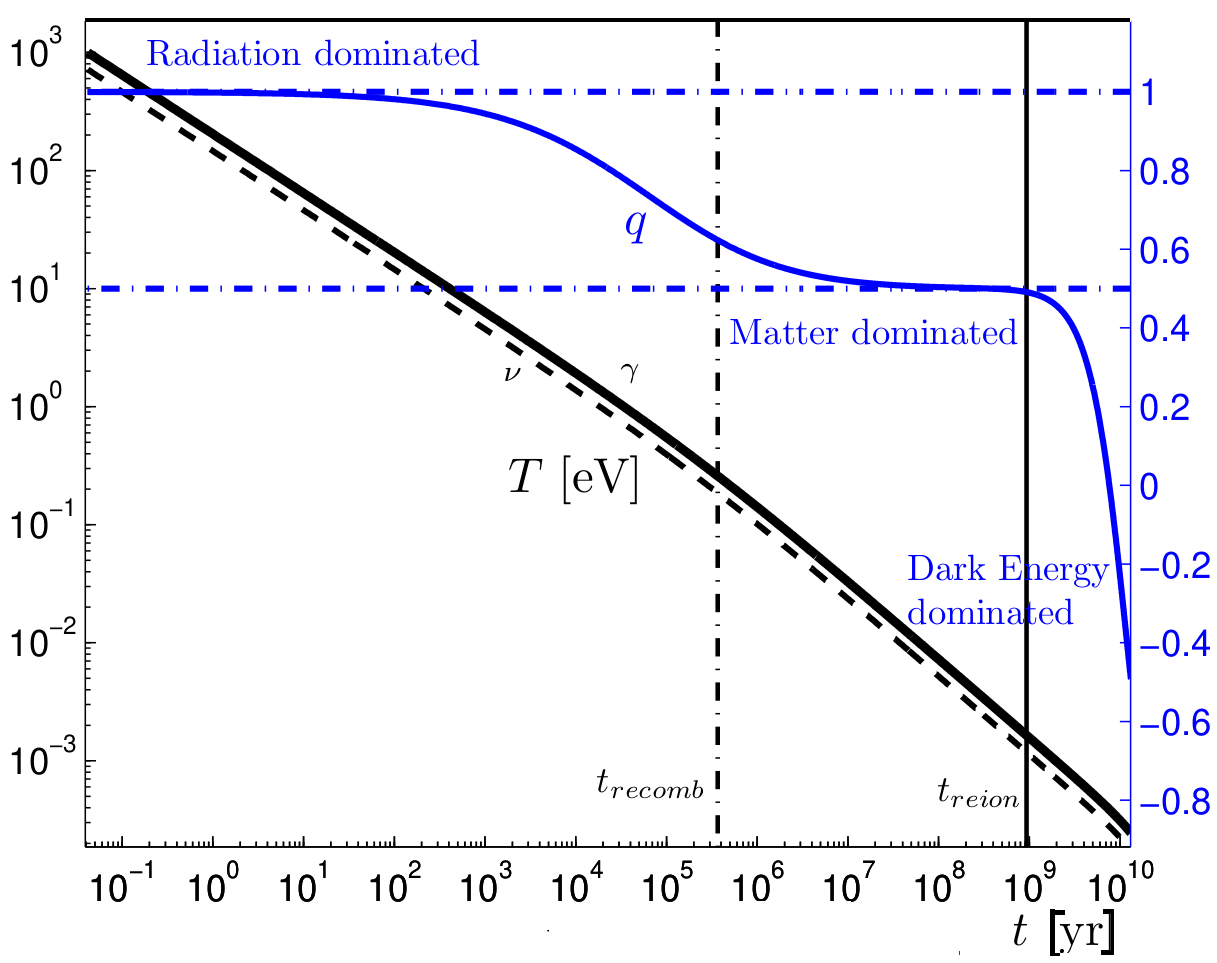
\includegraphics[width=0.75\linewidth]{plots/Tqtoday.png}}
\caption{Deceleration parameter (blue lines, right-hand scale) shows transitions in the composition of the Universe as a function of time. The left-hand scale indicates the corresponding temperature $T$, dashed is the lower $T$-value for neutrinos. Vertical lines indicate recombination and reionization conditions. \radapt{Rafelski:2013yka}.
\label{fig:today} }
\end{figure}
%%%%%%%%%%%%%%%%%%%%%%%%%%%%%%%%%%%%%%%

On the left-axis in~\rf{fig:today} we see temperature $T$\,[eV] while on right-axis (blue) we see the deceleration parameter $q$. The horizontal dot-dashed lines show the pure radiation-dominated value of $q=1$ and the matter-dominated value of $q=1/2$. The expansion in this era starts off as radiation-dominated. We see relatively long transitions to matter-dominated domain starting around $T=\mathcal{O}(300\eV)$ and ending at $T=\mathcal{O}(10\eV)$. The matter-dominated Universe\index{Universe!matter dominated} begins near recombination and ends right at the edge of reionization. Thereafter begins the transition to a dark energy $\Lambda$-dominated era which is in full swing already at $T=\mathcal{O}(1\eV)$. $q$ changes sign near to $T=\mathcal{O}(200\meV)$. Today $q=-0.5$ indicates we are in the midst of a rapid transition to dark energy $\Lambda$-dominated regime. 

The vertical dot-dashed lines in~\rf{fig:today} show the time of recombination at $T\simeq0.25\eV$, when the Universe became transparent to photons, and reionization at $T\simeq {\cal O}(1\meV)$, when hydrogen in the Universe was again ionized due to light from the first galaxies~\cite{Zaroubi:2012in} is also shown. The usefulness of $q$ to predict the present day value of the Hubble parameter\index{Hubble parameter} is even better appreciated noting that we can easily integrate~\req{eq:Hdot} 
\beqn\label{eq:HdotInt}
H(t)=\frac{H_i}{1+H_i\int_{t_i}^{t}(1+q)dt}=
\frac{H_i}{1+1.5\,H_i\int_{t_i}^{t}(1+P/\rho)dt}\,.
\eeqn
Given an initial (measured) value $H_i$ in an epoch after free electrons disappeared (recombination epoch) the time dependence of $q$ or equivalently, $P/\rho$, see~\rf{fig:today} impacts the current epoch $H(t_0)=H_0$. The Hubble parameter 
$H$\,[s$^{-1}$] (left ordinate, black) and the redshift $z$ (right ordinate, blue) 
\beqn\label{eq:zdef}
z+1\equiv \frac{a_0}{a(t)}\,,
\eeqn
are shown in~\rf{fig:today1} spanning a wide ranging domain following on the domain of interest in this work. 

%%%%%%%%%%%%%%%%%%%%%%%%%%%%%%%%%%%%%%%
\begin{figure}
\centerline{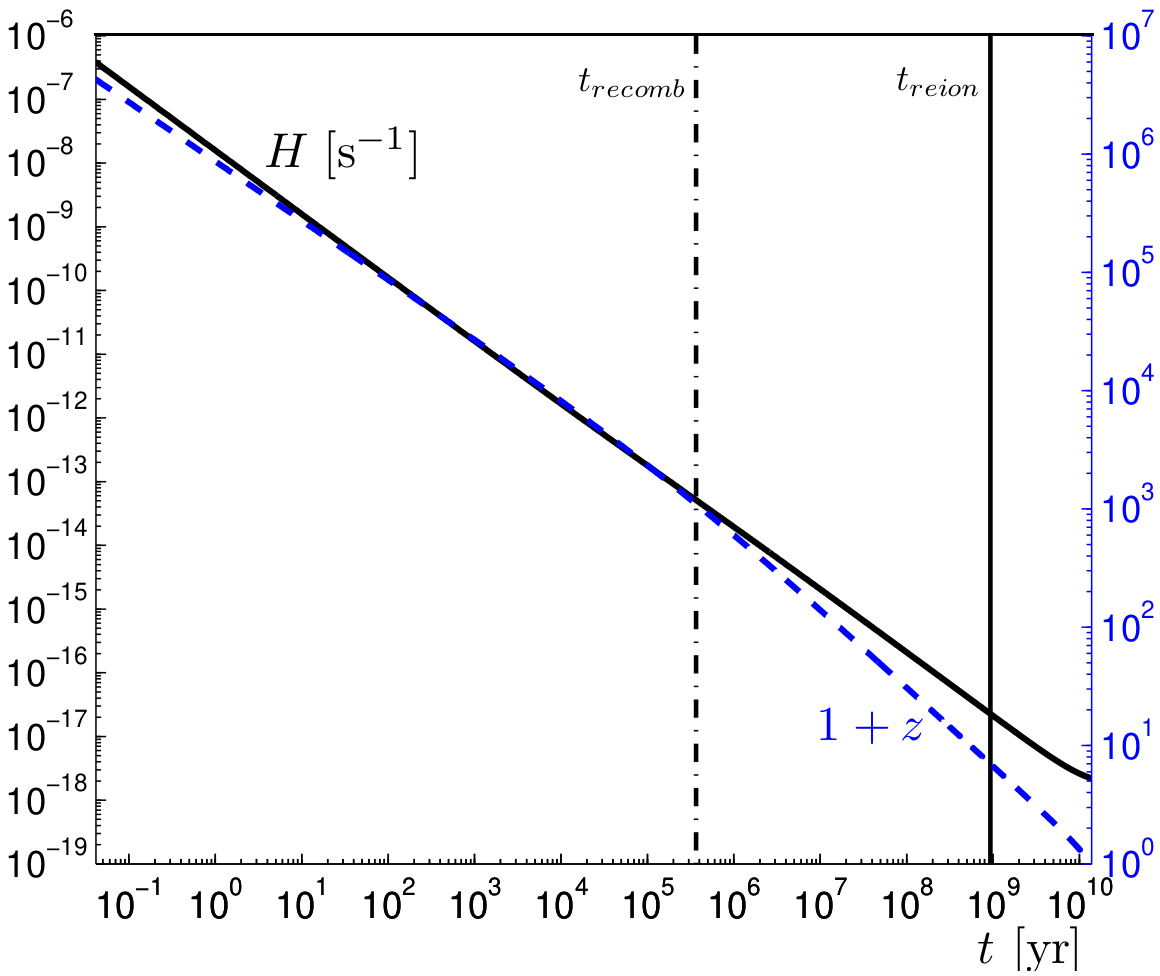
\includegraphics[width=0.65\linewidth]{plots/Hztoday.png}}
\caption{Temporal evolution of the Hubble parameter $H$ (in units 1/s] (left-hand scale) and of redshift $1+z$ (right-hand scale, blue). \radapt{Rafelski:2013yka}. 
\label{fig:today1} }
\end{figure}
%%%%%%%%%%%%%%%%%%%%%%%%%%%%%%%%%%%%%%%

There is a visible deviation from a power law behavior in~\rf{fig:today1} due to the transitions from radiation to matter dominated and from matter to dark energy dominated expansion we saw in~\rf{fig:today}. To achieve an increase $H$ in the current epoch beyond what is expected all it takes is to have the value of $q$ a bit more negative, said differently closer to being dark energy dominated altering the balance between matter, radiation (neutrinos, photons) and dark energy.\index{Universe!particle content} We conclude that it is important to understand the particle content of the Universe which we used to construct these results in order to understand the riddle of the Hubble value tension.\index{Hubble parameter!tension}

%%%%%%%%%%%%%%%%%%%%%%%%%%%%%
\para{Relation between time and temperature}
{\color{black} To determine the relation between time and temperature as the Universe evolves we first  consider} comoving entropy conservation\index{entropy!conservation}, 
\begin{align}
S=\sigma V\propto g^s_\ast T^3a^3=\mathrm{constant},
\end{align}
where $g^s_\ast$ is the entropy degree of freedom and $a$ is the scale factor. Differentiating the entropy with respect to time $t$ we obtain
\begin{align}
\left[\frac{\dot{T}}{g^s_\ast}\frac{dg^s_\ast}{dT}+3\frac{\dot{T}}{T}+3\frac{\dot{a}}{a}\right]g^s_\ast T^3a^3=0,\qquad \dot{T}=\frac{dT}{dt}.
\end{align}
The square bracket has to vanish. Solving for $\dot T $ we obtain
\begin{align}
\frac{dT}{dt}=-\frac{HT}{1+\frac{T}{3g^s_\ast}\frac{d\,g^s_\ast}{dT}}\,.
\end{align}
Taking the integral the relation between time and temperature in the primordial Universe is obtained\index{Universe!time-temperature relation}
\begin{align}\label{time}
t(T)=t_0-\int^T_{T_0} \frac{d\,T }{T\,H}\left[1+\frac{T}{3g^s_\ast}\frac{dg^s_\ast}{dT}\right],\qquad H=\sqrt{\frac{8\pi G_N}{3}\rho_{tot}(T)}
\,,
\end{align}
where $T_0$ and $t_0$ represent the initial temperature and time respectively. $H=\dot a/a$ is the Hubble parameter~\req{dynamic} related to the total energy density $\rho_{tot}$ in the Universe by the Hubble equation~\req{Hubble:eq} restated for convenience. The temperature derivative of the entropy degrees of freedom\index{entropy!degrees of freedom}, $g^\ast_s$ seen in~\rf{EntropyDOF:Fig} allows us to obtain a smooth time-temperature relation shown in~\rf{Fig:Overview}. We are using here the particle inventory in the Universe discussed earlier.

%%%%%%%%%%%%%%%%%%%%%%%%%%%%%%%%%%%%%%%
\begin{figure}
\centerline{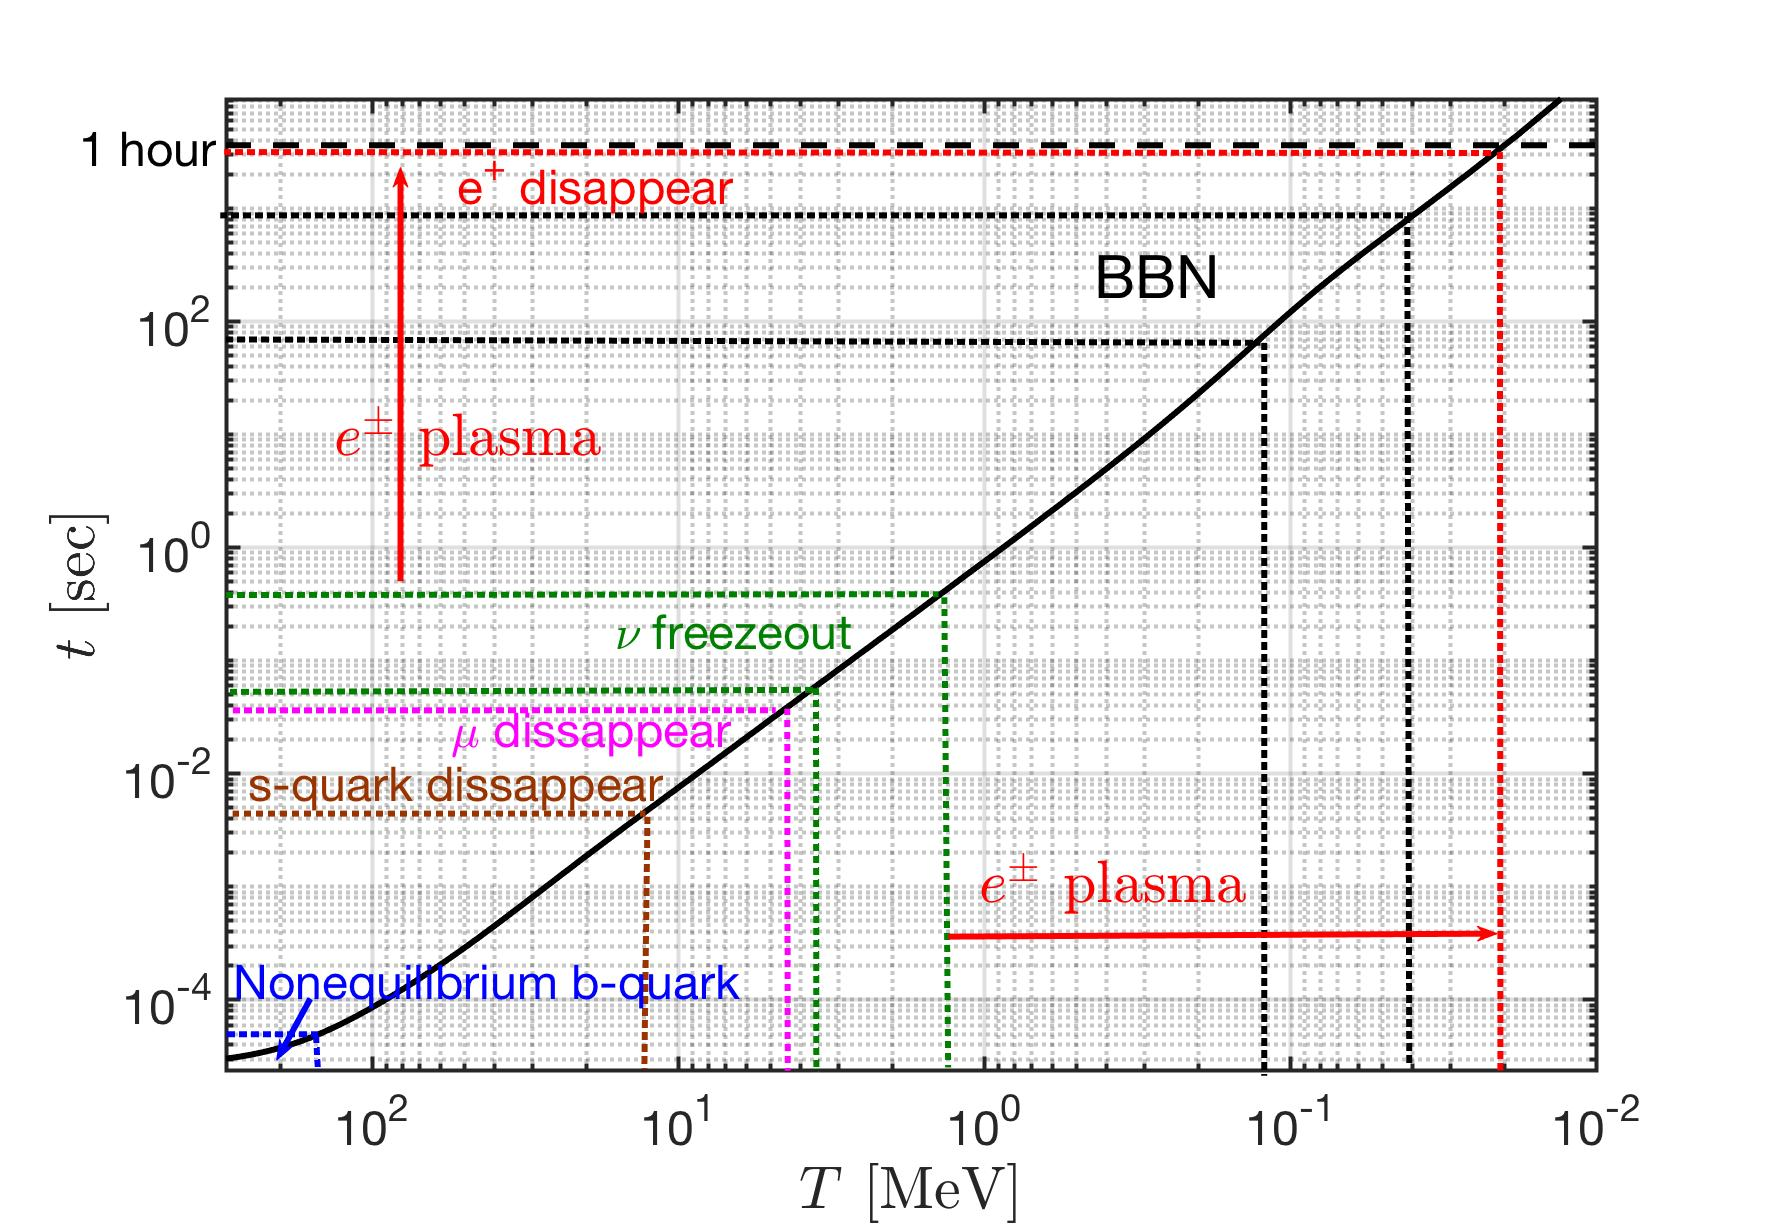
\includegraphics[width=0.85\linewidth]{plots/CosmicTimeTemperature.jpg}}
 \caption{The relation between time and temperature in the first hour of the Universe beginning shortly before QGP hadronization\index{QGP!hadronization} $300\MeV >T>0.02\MeV $ and ending with antimatter disappearance. Temperature/time range for several epochs is indicated. \radapt{Yang:2024ret}.}
 \label{Fig:Overview}
\end{figure}
%%%%%%%%%%%%%%%%%%%%%%%%%%%%%%%%%%%%%%%

In~\rf{Fig:Overview} the black line presents the computed relation between time $t$\,[s] (ordinate, increasing scale) and temperature $T$\,[MeV](abscissa, decreasing scale) during the first hour of the evolution of the Universe, reaching down to the temperature $T=10\keV$. Vertical and horizontal lines indicate some characteristic epochal events related to the Universe particle inventory, as marked. 

In the temperature range we consider in this work, $T>0.02\MeV$, particle-matter-radiation content of the Universe is relevant. There is vanishing dependence on $\Lambda$CDM model. However, in the contemporary Universe, the $\Lambda$CDM model uncertainties related to the lack of understanding of `darkness' and the need to know the pie-chart composition of the Universe at least at one `initial' time compound making in our view the direct measurements of $H_0$ a value that the extrapolations from recombination epoch should aim to resolve, eliminating the Hubble tension\index{Hubble parameter!tension}. Such a current epoch biased fit of data would provide as example the so called effective number of neutrino degrees of freedom that we address further below, see~\rsec{sec:model:ind}.


%%%%%%%%%%%%%%%%%%%%%%%%%%%%%%%%%%%%%%%%%
\para{Neutrinos in the cosmos}
%\label{ch:intro}
In the primordial Universe the neutrinos are kept in equilibrium with cosmic plasma via the weak interaction processes, which at temperatures below $\mathcal{O}(20)\MeV$ involve predominantly the $e^+e^-$-pair plasma. However, as the Universe expands, these weak interactions gradually became too slow to maintain equilibrium, neutrinos ceased interacting and decouple from the cosmic background as we describe in this report in detail in the temperature range $T=2.5\pm1.5\MeV$.

According to theoretical models we and others have developed, at around $1\MeV$ all cosmic neutrinos have stopped interacting. Neutrinos evolve as free-streaming\index{free-streaming} particles in the Universe responding only to gravitational background they co-create, as individual particles they are unlikely to interact again in the rapidly expanding and diluting Universe. Today they are the relic neutrino background.\index{neutrino!relic background} We recall that photons become free-streaming much later, near to $0.25$\,eV and today they make up the Cosmic Microwave Background (CMB), currently at a temperature\index{CMB} $T_{\gamma,0} =2.726\,\mathrm{K}=0.2349\MeV$.

The relic neutrino background carries important information about our primordial Universe: If we ever achieve relic neutrino experimental observation we will be observing our Universe when it was about $1$ sec old. Since photons were reheated by ensuing electron-positron annihilation, the neutrino relic background should have a lower temperature and we show below $T_\nu^0\simeq 1.95\,\mathrm{K}\simeq 0.168\MeV$ in the present epoch.
The relic neutrinos have not been directly measured, but their impact on the speed of expansion of the Universe is imprinted on the CMB. Indirect measurements of the relic neutrino background, such as by the Planck satellite~\cite{Planck:2018vyg,Planck:2015fie,Planck:2013pxb}, constrain to some degree in model dependent analysis the neutrino properties such as number of massless degrees of freedom and a bound on mass.

We know that the the neutrinos are not massless particles and we return to discuss how this insight was gained. Their square mass difference $\Delta m^2_{ij}$ has been\index{neutrino!mass} determined~\cite{ParticleDataGroup:2022pth}:
\begin{align}
&\Delta{m}_{21}^2=73.9\pm 2\MeV ^2,\\
&\Delta{m}_{32}^2=2450\pm 30\MeV ^2\,.
\end{align}
Thus neutrino mass\index{neutrino!mass} values can be ordered in the normal mass hierarchy ($m_1\ll m_2<m_3$) or inverted mass hierarchy ($m_3\ll m_1<m_2$). 

All three mass states remained relativistic until the temperature dropped below their rest mass. Today one of the neutrinos could be still relativistic. We will return in~\rsec{ch:nu:today} to discuss the relic massive neutrino flux in the Universe.
 
We will study the neutrino freeze-out\index{neutrino!freeze-out} temperature in the context of the kinetic Boltzmann-Einstein equation\index{Boltzmann-Einstein equation} for the three flavors, and refine the results by noting that there are three different freeze-out processes for neutrinos:
\begin{enumerate}
\item Neutrino chemical freeze-out: the temperature at which neutrino number changing processes such as $e^-e^+\to\nu\overline\nu$ effectively cease. After chemical freeze-out, there are no reactions that, in a noteworthy fashion, can change the neutrino abundance and so particle number is conserved.
%
\item Neutrino kinetic freeze-out: the temperature at which the neutrino momentum exchanging interactions such as $e^\pm\nu\to e^\pm\nu$ are no longer occurring rapidly enough to maintain an equilibrium momentum distribution. 
%
\item Collisions between neutrinos $\nu\nu\to\nu\nu$ are capable of re-equilibrating energy within and between neutrino flavor families. These processes end at a yet lower temperature and the neutrinos will be free-streaming from that point on.
\end{enumerate}

To obtain the freeze-out temperature $T=\mathcal{O}(2.5\pm1.5\mathrm{MeV})$, we solve the Boltzmann-Einstein equation including all required collision terms. To be able to do this
%with the transition matrices from Table.~\ref{T005} and Table.~\ref{T006}. 
%The properties of the neutrino background are influenced by the details of the freeze-out or decoupling process. 
we developed a new method for analytically simplifying the collision integrals and showing that the neutrino freeze-out temperature is controlled by one fundamental coupling constants and particle masses. We give further discussion of these methods in~\rsec{ch:param:studies}. The required mathematical theory and numerical method is developed in Appendices~\ref{ch:vol:forms}, \ref{ch:boltz:orthopoly}, and \ref{ch:coll:simp}. Our report follows the comprehensive investigation of neutrino freeze-out found also in Jeremiah Birrell PhD thesis~\cite{Birrell:2014ona}.\index{neutrino!freeze-out}

The freeze-out temperature we obtain depends only on the magnitude of the symmetry breaking Weinberg angle $\sin^2(\theta_W)$, and a dimensionless relative interaction strength parameter $\eta$,
\begin{align}\label{etaCTY}
\eta\equiv M_p m_e^3 G_F^2, \qquad M_p\equiv\sqrt{\frac{1}{8\pi G_N}}\,, 
\end{align}
a combination of the electron mass $m_e$, Newton constant $G_N$ (expressed above in terms of Planck mass $M_p$,~\req{eq:GN}), and the Fermi constant $G_F$. These dimensionless strength parameters in the present-day vacuum state have the following values
\begin{align}\label{eta0CTY}
\eta_0\equiv \left.M_p m_e^3 G_F^2\right|_0 = 0.04421\,, \qquad \sin^2(\theta_W)=0.2312\,.
\end{align}

The magnitude of neither $\eta$ nor of the Weinberg angle is fixed by known phenomena. Therefore both the interaction strength $\eta$ and $\sin^2(\theta_W)$ could be subject to variation as a function of time or temperature. Therefore it is of interest to study the neutrino freeze-out as function of these parameters. The dependence of neutrino freeze-out temperatures on $\eta$ is shown in~\rf{fig:freeze-outT_eta} and the dependence on the Weinberg angle is shown in~\rf{fig:freeze-outT_B}. The present day vacuum value of Weinberg angle puts the $\nu_\mu,\nu_\tau$ freeze-out temperature, seen in the right hand frame of \rf{fig:freeze-outT_B}, near its maximum value.
 
%%%%%%%%%%%%%%%%%%%%%%%%%%%%%%%%%%%%%%%
\begin{figure}
\centerline{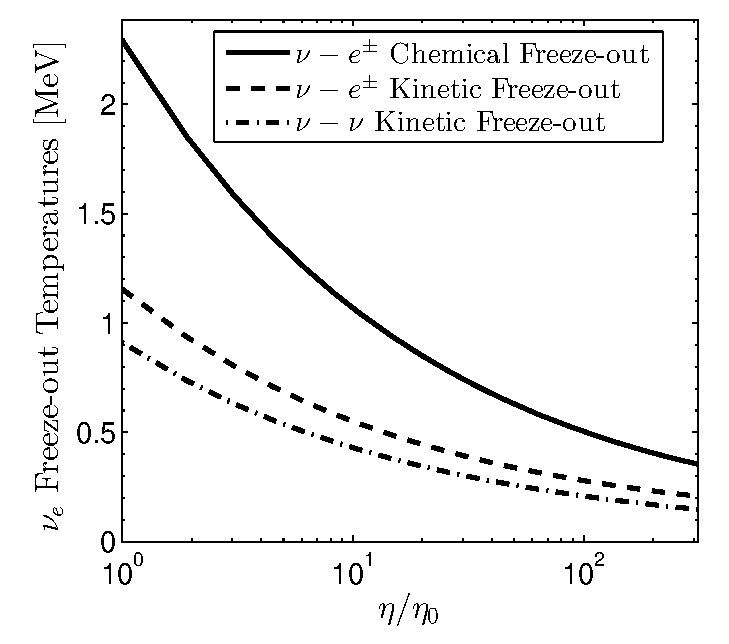
\includegraphics[width=0.49\linewidth]{plots/nu_e_freezeout_GF.pdf} 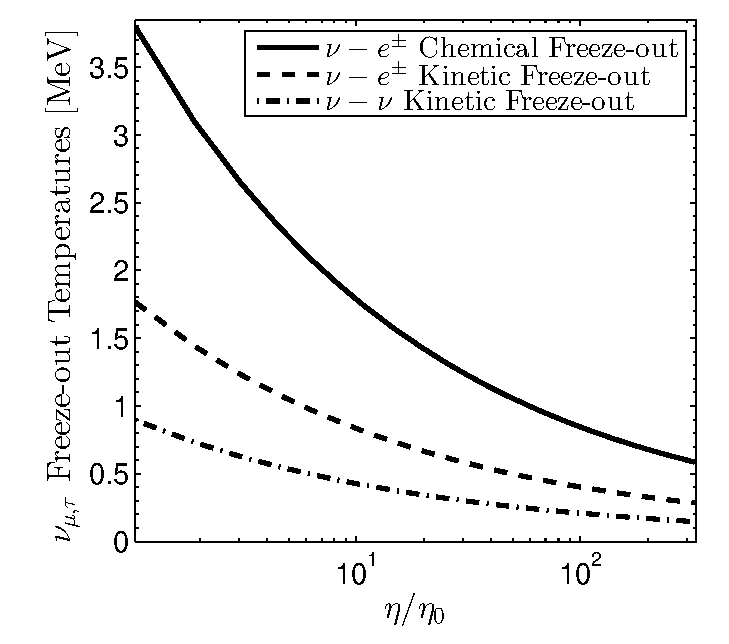
\includegraphics[width=0.49\linewidth]{plots/nu_mu_freezeout_GF.pdf}}
\caption{Freeze-out temperatures for electron neutrinos (left hand frame) and $\mu$, $\tau$ neutrinos (right hand frame) for the three types of processes, see insert, as functions of interaction strength $\eta>\eta_0$. \cccite{Birrell:2014uka}}
\label{fig:freeze-outT_eta}
 \end{figure}
%%%%%%%%%%%%%%%%%%%%%%%%%%%%%%%%%%%%%%%


%%%%%%%%%%%%%%%%%%%%%%%%%%%%%%%%%%%%%%%
\begin{figure}
\centerline{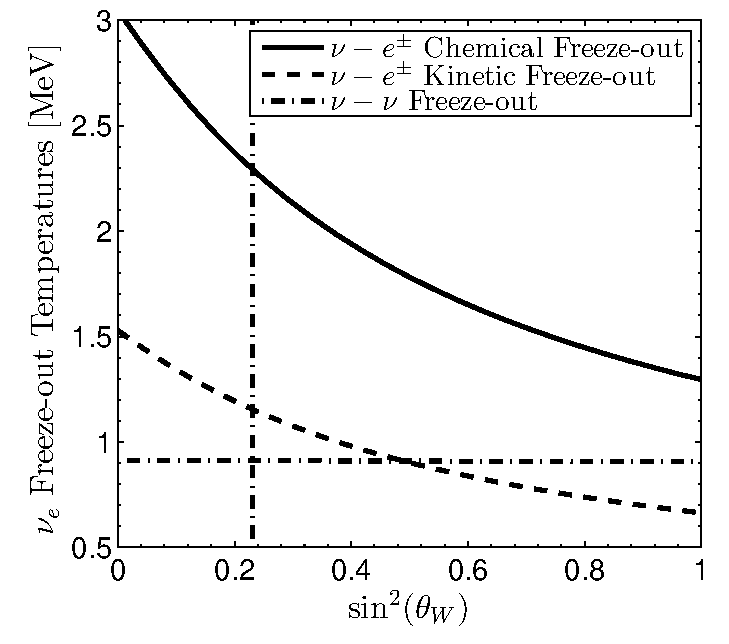
\includegraphics[width=0.49\linewidth]{plots/nu_e_freezeout.pdf}
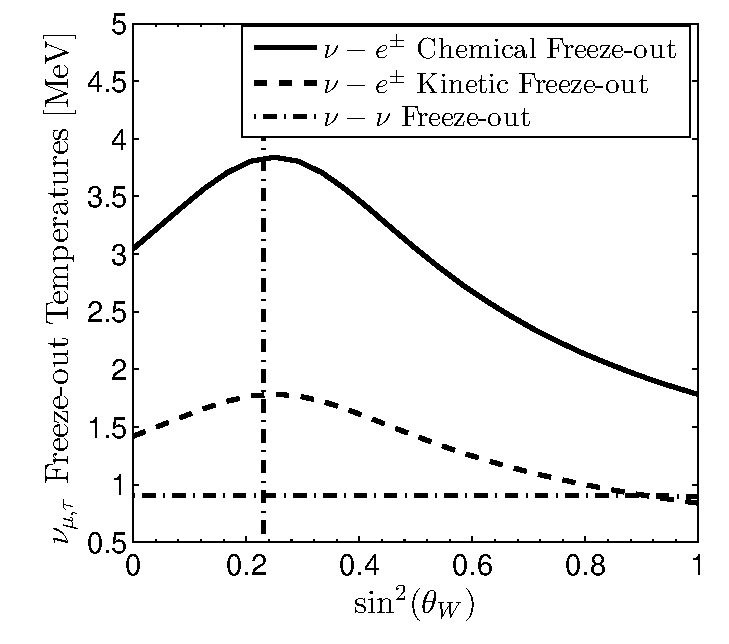
\includegraphics[width=0.49\linewidth]{plots/nu_mu_freezeout.pdf}}
\caption{Freeze-out temperatures for electron neutrinos (left hand frame) and $\mu$, $\tau$ neutrinos (right hand frame) for three types of processes, see insert, as functions of the value of the Weinberg angle $\sin^2(\theta_W)$. Vertical line is at present epoch $\sin^2(\theta_W)=0.23$. \cccite{Birrell:2014uka}}
\label{fig:freeze-outT_B}
 \end{figure}
%%%%%%%%%%%%%%%%%%%%%%%%%%%%%%%%%%%%%%%

We do not explore here the pivotal insight that neutrinos in elementary processes are not produced in mass eigenstates but in flavor eigenstates. Due to the difference in the three neutrino masses the propagating flavor eigenstates contain three coherent amplitudes moving at different velocity. This leads to the experimentally observed oscillation of neutrino flavor as function of travel distance.\index{neutrino!flavor oscillation} This is also how the constraints on neutrino masses shown above were obtained.

How does this neutrino mixing impact neutrino freeze-out? We inspect our results to understand the hierarchy of freeze-out: Near to freeze-out temperature the electron-neutrino can still `annihilate' on electrons while the absence of muons and taus in the cosmic plasma at a temperature of a few MeV makes these two neutrino flavors less interactive and their freeze-out temperature is higher. Oscillation thus provides a mechanism in which the heavier flavors remain reactive in matter as they share in the more interactive electron-neutrino component. Conversely, electron-neutrino interaction is weakened since only a part of this flavor wave remains available to interact. The net effect was found negligible in the work of Mangano et. al.~\cite{Mangano:2005cc}. The impact of the cosmic magnetic field on neutrino oscillation is an avenue for further research~\cite{Rafelski:2023zgp}.

In regard to our results one can say that the differences in freeze-out between the three different flavors diminishes allowing for oscillations. We chose not to quantify this effect as the mixing of neutrino mass eigenstates into flavor eigenstates and neutrino masses remain a vibrant research field. Without knowing all the required input parameters the outcome is uncertain. Given the results we obtained and methods we developed we will be able, once the neutrino mixing and masses are well understood, to update our results. 

A discussion of the implications and connections of the results on neutrino freeze-out to other areas of physics, including BBN\index{Big-Bang!BBN} and dark radiation is described in more detail in~\cite{Birrell:2014uka,Dreiner:2011fp,Boehm:2012gr,Blennow:2012de}. 

We now characterize the era $30\MeV>T>0.01\MeV$. At the high end muons\index{muon} and pions are nonrelativistic and are disappearing from the Universe, we then pass through neutrino decoupling and the era where $e^+e^-$-pairs become nonrelativistic. In~\rf{fig:BBN} the black line refers to the left ordinate and shows the temperature as a function of time, dashed the lower value of $T$ for free-streaming neutrinos. We further indicate in~\rf{fig:BBN} the domain of Big-Bang Nucleosynthesis (BBN)~\cite{Iocco:2008va}\index{Big-Bang!BBN}, the period when the lighter elements were synthesized amidst of a $e^+e^-$-pair plasma, which is already reduced in abundance but not entirely eliminated. This insight will keep us very busy in this report. 


%%%%%%%%%%%%%%%%%%%%%%%%%%%%%%%%%%%%%%%
\begin{figure}
\centerline{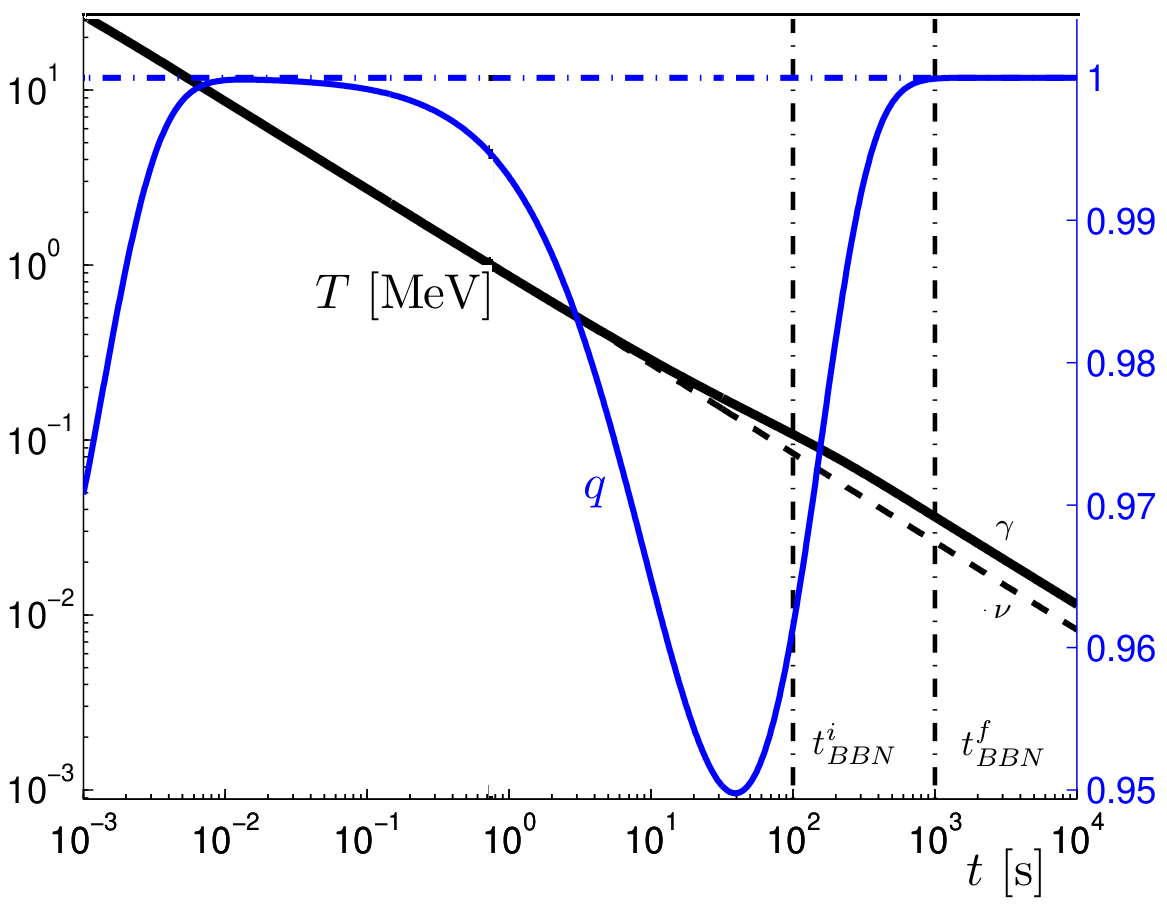
\includegraphics[width=0.60\linewidth]{plots/TqBBN.png}}
\caption{The first hours in the lifespan of the Universe from the end of baryon antimatter annihilation through BBN: Deceleration parameter\index{cosmology!deceleration parameter} $q$ (blue line, right-hand scale) shows impact of emerging antimatter components; at millisecond scale anti-baryonic matter and at 35\,sec. scale positronic nonrelativistic matter appears. The left-hand scale shows photon $\gamma$ temperature $T$ in\,eV, dashed is the emerging lower value for neutrino $\nu$ which are not reheated by $e^+e^-$ annihilation. Vertical lines bracket the BBN domain. \cccite{Birrell:2014uka}. \radapt{Rafelski:2013yka}} 
\label{fig:BBN}
\end{figure}
%%%%%%%%%%%%%%%%%%%%%%%%%%%%%%%%%%%%%%%

The blue lines in~\rf{fig:BBN} refer to the right ordinate: The horizontal dot-dashed line for $q=1$ shows the pure radiation dominated value with two exceptions. In~\rf{fig:BBN} the unit of time is seconds and the range spans the domain from fractions of a millisecond to a few hours.

The just noted presence of massive pions and muons reduces the value of $q$ towards matter dominated near to the maximal temperature shown. Second, when the temperature is near the value of the electron mass, the $e^+e^-$-pairs are not yet fully depleted but already sufficiently nonrelativistic to cause another dip in $q$ towards matter-dominated value. These dips in $q$ are not large; the Universe is still predominantly radiation-dominated.\index{acceleration parameter} But $q$ provides a sensitive measure of when various mass scales become relevant and is therefore a good indicator for the presence of a reheating period, where some particle population disappears and passes its entropy to the thermal background.

%%%%%%%%%%%%%%%%%%%%%%%%%%%%%%%%%%%%%%%%%%%%
\para{Reheating history of the Universe}%\label{Eralink}
At times where dimensional scales are irrelevant, entropy conservation\index{entropy!conservation} means that temperature scales inversely with the scale factor $a(t)$. This follows from the only contributing scale being $T$ and therefore by dimensional counting $ \rho\simeq 3P \propto T^4$. However, as the temperature drops and at their respective $m\simeq T$ scales, successively less massive particles annihilate and disappear from the thermal Universe. Their entropy reheats the other degrees of freedom and thus in the process, the entropy originating in a massive degree of freedom is shifted into the effectively massless degrees of freedom that still remain. 

This causes the $T\propto 1/a(t)$ scaling to break down; during each of these `reorganization' periods the drop in temperature is slowed by the concentration of entropy in fewer degrees of freedom, leading to a change in the reheating ratio, $R$, defined as\index{reheating}
\begin{equation}\label{redshiftratio}
R\equiv \frac{1+z}{ T_\gamma/T_{\gamma,0}}, \qquad 1+z\equiv \frac{a_{0}}{a(t)}.
\end{equation}
The reheating ratio connects the photon temperature redshift to the geometric redshift, where $a_0$ is the scale factor today (often normalized to $1$) and quantifies the deviation from the scaling relation between $a(t)$ and $T$. There is additional Universe expansion due to reheating of remaining degrees of freedom so that the total entropy is conserved as entropy in particles decreases. This is Universe reheating inflation.\index{Universe!reheating inflation}

The change in $R$ can be computed by the drop in the number of degrees of freedom and we learn from this actual redshift $1+z$. For the just discussed era $30\MeV>T>0.01\MeV$, we show in~\rf{fig:BBN1} in blue the value of $1+z$ as a function of time and in black (left ordinate) the value of $H$[s$^{-1}$]. It is interesting to observe that study of BBN\index{BBN!redshift} extends the range of redshift explored to $10^8<1+z_\mathrm{BBN}<10^9$.

%%%%%%%%%%%%%%%%%%%%%%%%%%%%%%%%%%%%%%%
\begin{figure}
\centerline{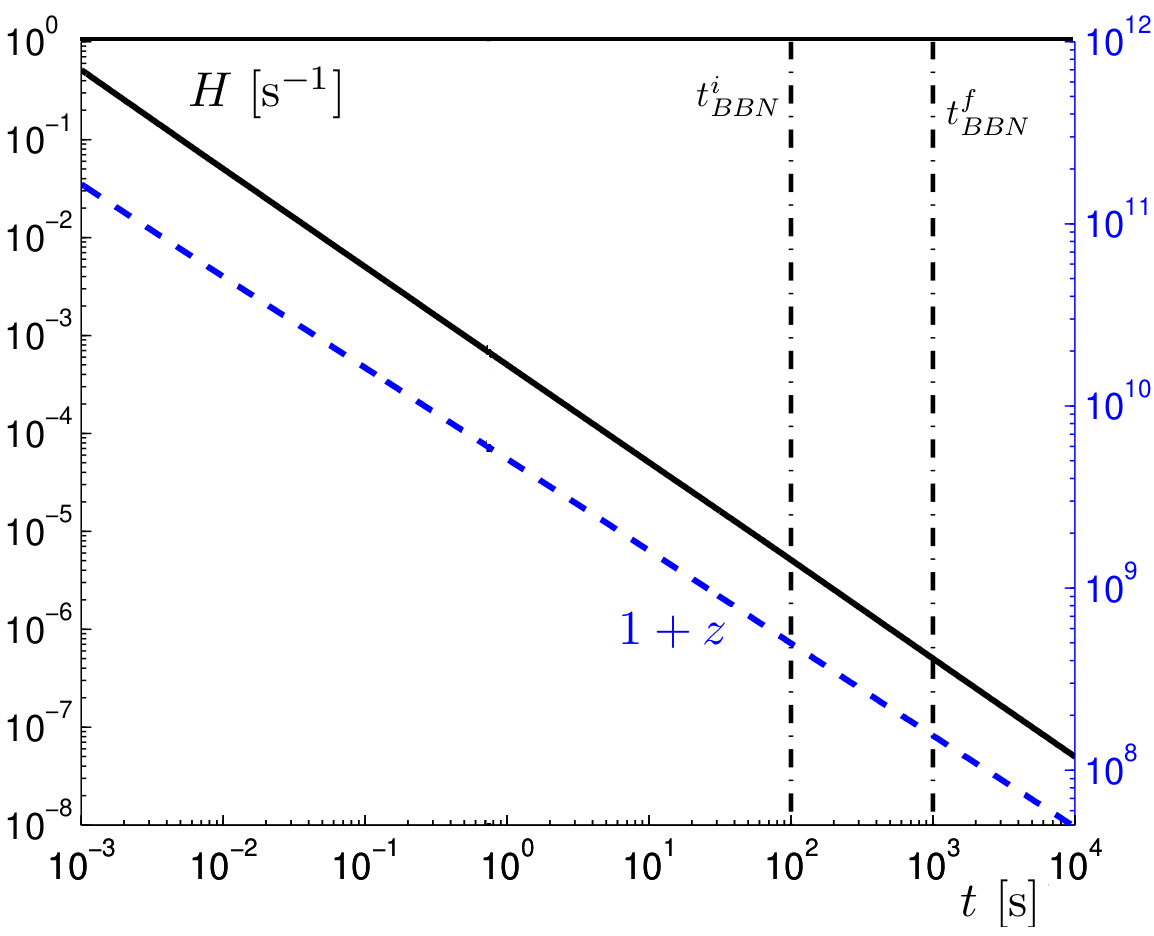
\includegraphics[width=0.60\linewidth]{plots/HzBBN.png}} 
\caption{First hours in the evolution of the Universe: Hubble parameter $H$ in units [1/s] (left-hand scale) and the redshift $1+z$ (right-hand scale, blue) spanning the epoch from well below the end of baryon antimatter annihilation through BBN, compare~\rf{fig:BBN}.\index{reheating!inflation} \radapt{Rafelski:2013yka}. \cccite{Birrell:2014uka}} \label{fig:BBN1}
\end{figure}
%%%%%%%%%%%%%%%%%%%%%%%%%%%%%%%%%%%%%%%

We are interested in determining by how much the Universe inflated in addition to its expected expansion in follow-up on particle disappearance from inventory. We begin at the highest temperature to count the particle degrees of freedom: At a temperature on the order of the top quark mass, when all standard model particles were in thermal equilibrium, the Universe was pushed apart by 28 bosonic and 90 fermionic degrees of freedom. The total number of degrees of freedom can be computed as discussed below. 

For bosons we have the following: the doublet of charged Higgs\index{Higgs} particles has $4=2\times2=1+3$ degrees of freedom -- three will migrate to the longitudinal components of $W^\pm, Z$ when the electro-weak vacuum freezes and the EW symmetry breaking arises\index{symmetry!breaking}, while one is retained in the one single dynamical charge-neutral Higgs particle component. In the massless stage, the SU(2)$\times$U(1) theory has 4$\times$2=8 gauge degrees of freedom where the first coefficient is the number of particles $(\gamma, Z, W^\pm)$ and each massless gauge boson has two transverse conditions of polarization. Adding in $8_c\times2_s=16$ gluonic degrees of freedom we obtain 4+8+16=28 bosonic degrees of freedom. 

The count of fermionic degrees of freedom includes three $f$ families, two spins $s$, another factor two for particle-antiparticle duality. We have in each family of flavors a doublet of $2\times 3_c$ quarks, 1-lepton and 1/2 neutrinos (due left-handedness which was not implemented counting spin). Thus we find that a total $3_f\times 2_p\times 2_s\times(2\times 3_c+1_l+1/2_\nu)=90$ fermionic degrees of freedom. We further recall that massless fermions contribute 7/8 of that of bosons in both pressure and energy density. Thus the total number of massless Standard Model particles at a temperature above the top quark mass scale, referring by convention to bosonic degrees of freedom, is $g_{\rm SM}=28+90\times 7/8=106.75$\,.

In~\rf{fig:dof} we show the reheating ratio $R$ \index{Universe!reheating inflation}~\req{redshiftratio} as a function of time beginning in the primordial elementary particle Universe epoch on the left, connecting to the present epoch on the right. The periods of change seen in~\rf{fig:dof} come when the evolution temperature crosses the mass of a particle species that is in equilibrium. One can see drops corresponding to the disappearance of thermal particle yields as indicated. After $e^+e^-$ annihilation on the right, there are no significant degrees of freedom remaining to annihilate and feed entropy into photons, and so $R$ remains constant until today. We do not model in detail the QGP phase transition and hadronization\index{QGP!hadronization} period near $T\simeq O(150\,\MeV), t\simeq 20\,\mu\mathrm{s}$ covering-up the resultant kinky connection. A more precise model using lattice QCD, see \eg~\cite{Borsanyi:2013bia}, together with a high temperature perturbative QCD expansion, see \eg~\cite{Letessier:2002ony}, can be considered. These complex details do not impact this study and so we do not consider these issues further here.

%%%%%%%%%%%%%%%%%%%%%%%%%%%%%%%%%%%%
%\begin{sidewaysfigure}height=0.35\linewidth,
\begin{figure}
%\vspace*{0.65\linewidth}
{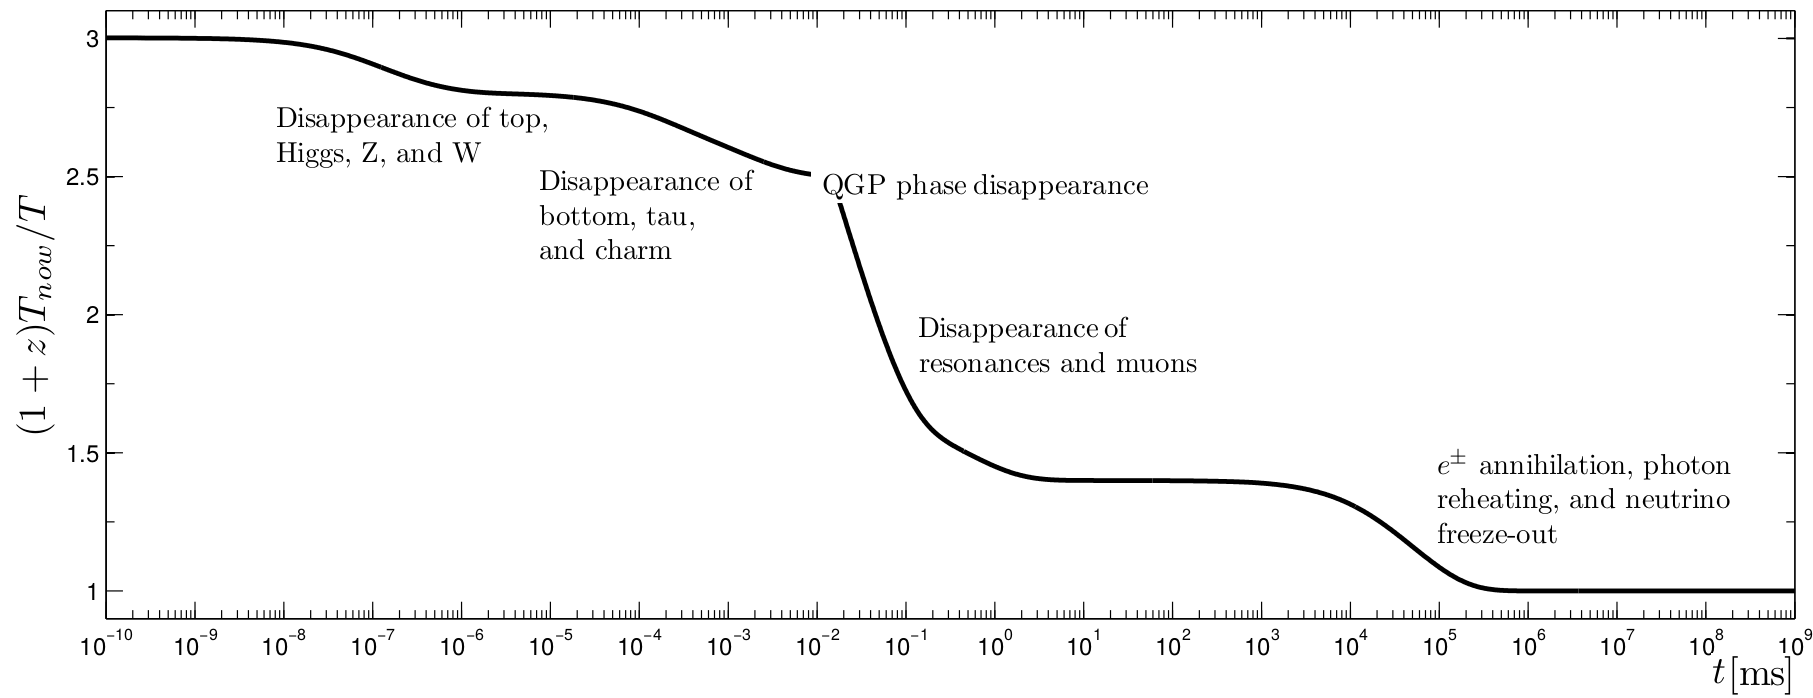
\includegraphics[width=\linewidth]{plots/DOFtime.png}}
\caption{Universe inflation due to the disappearance of degrees of freedom as a function of time $t$\,[ms] (milliseconds). The Universe volume inflated by approximately a factor of 27 above the naive thermal redshift scale as massive particles disappeared successively from the inventory while entropy remained conserved. \radapt{Birrell:2014ona}}\label{fig:dof}
%\end{sidewaysfigure}
\end{figure}
%%%%%%%%%%%%%%%%%%%%%%%%%%%%%%%%%%%%

As long as the microscopic local dynamics are at least approximately entropy conserving, the total drop in $R$ is entirely determined by the global entropy conservation governing expansion of the Universe based on FLRW\index{cosmology!FLRW} cosmology. Namely, the magnitude of the drop in $R$ seen in~\rf{fig:dof} is a measure of the number of degrees of freedom that have disappeared from the Universe. Consider two times $t_1$ and $t_2$ at which all particle species that have not yet annihilated are effectively massless. By conservation of comoving entropy and scaling $T\propto 1/a$ we have
\begin{equation}\label{r_ratio}
1=\frac{a_1^3S_{1}}{a_2^3 S_2}=\frac{a_1^3\sum_ig_i T_{i,1}^3}{a_2^3\sum_j g_j T_{j,2}^3},\qquad \left(\frac{R_1}{R_2}\right)^3=\frac{\sum_ig_i (T_{i,1}/T_{\gamma,1})^3}{\sum_j g_j (T_{j,2}/T_{\gamma,2})^3}
\,,
\end{equation}
where the sums are over the total number of degrees of freedom present at the indicated time and the degeneracy factors $g_i$ contain the $7/8$ factor for fermions. In the second form we divided the numerator and denominator by $a_{0}T_{\gamma,0}$. 

We distinguish between the temperature of each particle species and our reference temperature, the photon temperature. This is important since today neutrinos are colder than photons, due to photon reheating from $e^+e^-$ annihilation occurring after neutrinos decoupled (this is only an approximation, a point we will study in detail in subsequent chapters). By conservation of entropy one obtains the neutrino to photon temperature ratio of
\begin{equation}\label{T_nu_T_gamma}
T_\nu/T_\gamma=({4}/{11})^{1/3}.
\end{equation}
We will call this the reheating ratio in the decoupled limit. 

We now compute the total drop in $R$ shown in~\rf{fig:dof}. At $T=T_\gamma=\mathcal{O}(130\GeV)$ the number of active degrees of freedom is slightly below $g_{\rm SM}=106.75$ due to the partial disappearance of top quarks $t$ which have mass $174\,\GeV$, but this approximation will be good enough for our purposes. At this primordial time, all the species are in thermal equilibrium with photons.

Today we have $2$ photon and $7/8\times 6$ neutrino degrees of freedom and a neutrino-to-photon temperature ratio~\req{T_nu_T_gamma}. Therefore, for the overall reheating ratio since the primordial elementary particle Universe epoch we have\index{Universe!reheating}
\begin{equation}
\left(\frac{R_{100GeV}}{R_{now}}\right)^3= \frac{g_{SM}}{g_{\rm now}}=\frac{106.75}{2+\frac{7}{8}\times 6\times \frac{4}{11}}\approx 27.3
\end{equation}
which is the fractional change we see in~\rf{fig:dof}. The meaning of this factor is that the Universe approximately inflated by a factor 27 above the thermal redshift scale as massive particles disappeared successively from the inventory. 

Another view of the reheating is implicit in our presentation of particle energy inventory in~\rf{fig:energy:frac}. There the initial highest temperature is on the right at the end of the hadron era marked by the disappearance of muons and pions and other heavier particles as marked. This constitutes a major reheating period, with energy and entropy from these particles being transferred to the remaining $e^+e^-$, photon, neutrino plasma. Continuing to $T=\mathcal{O}(1)\MeV$, we come to the annihilation of $e^+e^-$ and the photon reheating period. Notice that only the photon energy density fraction increases here. As discussed above, a common simplifying assumption is that neutrinos are already decoupled at this time and hence do not share in the reheating process, leading to a difference in photon and neutrino temperatures~\req{T_nu_T_gamma}.

After passing through a long period, from $T=\mathcal{O}(1)\MeV$ until $T=\mathcal{O}(1)$\,eV, where the energy density is dominated by photons and free-streaming neutrinos, we then come to the beginning of the matter dominated regime, where the energy density is dominated by dark matter and baryonic\index{baryon} matter. This transition is the result of the redshifting of the photon and neutrino de Broglie wavelength and hence particle energy, for relativistic particles $\rho\propto T^4$, whereas for nonrelativistic matter $\rho\propto a^{-3}\propto T^3$. Note that our inclusion of neutrino mass\index{neutrino!mass} causes the leveling out of the neutrino energy density fraction during this period, as compared to the continued redshifting of the photon energy.

Finally, as we move towards the present day CMB\index{CMB} temperature of $T_{\gamma,0}=0.235$ meV on the left-hand side, we have entered the dark energy dominated regime. For the present day values, we have used the fits from the Planck data~\cite{Planck:2018vyg,Planck:2015fie,Planck:2013pxb} of $69\%$ dark energy, $26\%$ dark matter and $5\%$ baryons (and zero spatial curvature). The photon energy density is fixed by the CMB temperature $T_{\gamma,0}$ and the neutrino energy density is fixed by $T_{\gamma,0}$ along with the photon to neutrino temperature ratio. Both constitute $<1\%$ of the current energy budget in the pie chart of the Universe.


%%%%%%%%%%%%%%%%%%%%%%%%%%%%%
\para{The baryon-per-entropy density ratio}
An important\index{baryon!entropy ratio}
result of the FLRW cosmology is that following on the era of matter genesis both baryon and entropy content is conserved in the comoving volume, that is the volume where length scales account for the Universe $a(t)$ expansion scale parameter. Therefore the ratio of baryon number density to visible matter entropy density remains constant throughout the evolution of the thermally equilibrated Universe. 

Baryonic dust floating in the Universe dilutes due to volume growth with the $a(t)^3$ factor. The entropy described using the entropic degrees of freedom $g^\ast_s$ seen in~\rf{EntropyDOF:Fig} scales overall with the third power of Temperature and thus with the third power of the same expansion parameter, $a(t)^3$. During the short epochs when mass matters, scattering allows the disappearing massive particles to transfer their entropy to the remaining thermal background such that the scale parameter $a(t)$ inflates in each period of reheating, see prior discussion. 

{\color{black} By these considerations,} we have\index{baryon!entropy ratio}
\begin{align}
\frac{n_B-n_{\overline{B}}}{\sigma}= \left.\frac{n_B-n_{\overline{B}}}{ \sigma}\right|_{t_0}=\mathrm{Const.}\;
\end{align}
The subscript $t_0$ denotes the present day condition, and $\sigma$ is the total entropy density.
The observation gives the present baryon-to-photon\index{baryon!per photon ratio} ratio~\cite{ParticleDataGroup:2022pth} $5.8 \times 10^{-10} \leqslant(n_B-n_{\overline{B}})/n_\gamma\leqslant6.5\times10^{-10}$. This small value quantifies the matter-antimatter asymmetry in the present day Universe, and allows the determination of the present value of baryon per entropy ratio~\cite{Rafelski:2019twp,Fromerth:2002wb,Fromerth:2012fe}:
\begin{align}\label{BaryonEntropyRatio}
\left.\frac{n_B-n_{\overline{B}}}{ \sigma}\right|_{t_0}=\eta_\gamma\left(\frac{n_\gamma}{\sigma_\gamma+\sigma_\nu}\right)_{\!t_0}\!\!\!\!=(8.69\pm0.05)\!\!\times\!\!10^{-11},\qquad \eta_\gamma=\frac{(n_B-n_{\overline{B}})}{n_\gamma},
\end{align}
where the value $\eta_\gamma=(6.14\pm0.02)\times10^{-10}$~\cite{ParticleDataGroup:2022pth} is used in calculation. 

To obtain the above ratio, we have considered the Universe today to be containing photons and free-streaming massless neutrinos~\cite{Birrell:2012gg}, and $\sigma_\gamma$ and $\sigma_\nu$ are the entropy densities for photon and neutrino respectively. We have
\begin{align}
 \frac{\sigma_\nu}{\sigma_\gamma}=\frac{7}{8}\,\frac{g_\nu}{g_\gamma}\left(\frac{T_\nu}{T_\gamma}\right)^3\,,\qquad\frac{T_\nu}{T_\gamma}=\left(\frac{4}{11}\right)^{1/3}
 \,,
\end{align}
and the entropy-per-particle\index{entropy!per particle} for massless bosons and fermions are given by~\cite{Fromerth:2012fe}
\begin{align}
\sigma/n|_\mathrm{boson}\approx 3.60\,,\qquad
\sigma/n|_\mathrm{fermion}\approx 4.20\,.
\end{align}
The evaluation of entropy of free-streaming fluid in terms of effectively massless $m\,a_f/a(t)$ free-streaming particles (neutrinos) needs further consideration, as does the free-streaming particles entropy definition. We will return to consider these very important questions in the near future.
